\documentclass{jps-cp}
\usepackage{txfonts} %Please comment out this line unless the txfonts package is availabe in your LaTeX system.
\usepackage[dvipdfmx]{graphicx}
%\usepackage[dvipdfmx]{graphicx}
%\usepackage[dvipdfmx]{color}
%\documentclass[onecolumn]{preport}
% \usepackage{comment}
% \usepackage{amsmath}
% \usepackage{bm}
%\graphicspath{{figs/}}

\title{Development and  of Iron Thin Films for Polarization Analysis of Ultracold Neutrons}

\author{Hanako \textsc{Butsuri}$^{1}$ and Taro \textsc{Butsuri}$^{2}$}

\inst{$^{1}$Physical Society of Japan, 2-31-22-5F Yushima, Bunkyo, Tokyo 113-0034, Japan \\
$^{2}$JPSJ Editorial Division, Physical Society of Japan, 2-31-22-5F Yushima, Bunkyo, Tokyo 113-0034, Japan}

\email{jpsj{\_}edit@jps.or.jp}

\recdate{February 21, 2019}

\abst{
The TUCAN (TRIUMF Ultra-Cold Advanced Neutron) collaboration aims  to search for the neutron electric dipole moment (nEDM) with unprecedented precision. 
One of the essential elements for this nEDM measurement is a polarization analyzer of ultracold neutrons (UCN), which is based on a spin-dependent potential of UCNs as they pass through a magnetized iron film. This iron film is required to be saturated by a small applied magnetic field of about 10~mT. In this work, samples of thin iron films sputtered on aluminum or silicon substrates were fabricated using the Ion Beam Sputtering (IBS) facility at the Institute for Integrated Radiation and Nuclear Science, Kyoto University (KURNS), and were characterized by Vibrating Sample Magnetometry (VSM) and cold-neutron reflectometry.
As a result, the samples on aluminum substrates were found to be saturated by an applied magnetic field of about 15~mT, and those on  silicon substrates were found to produce a magnetic potential of neutrons corresponding to about 2.0~T by a magnetic field of about 8~mT. These performances are sufficient to be used for a UCN polarization analyzer.}
\kword{keyword1, keyword2, keyword3, \ldots}

\begin{document}
\maketitle

\section{Introduction}
\subsection{Background}

The presence of a finite neutron electric dipole moment (nEDM) would violate time-reversal symmetry. This is equivalent to CP violation 

nEDM measurements place severe constraints on the search for time-reversal symmetry breaking and on theories beyond the Standard Model. The existence of nEDM breaks the time-reversal symmetry, and assuming CPT symmetry, the breaking of % time-reversal symmetry is equivalent to the breaking of 
The size of the nEDM is expected to be $10^{-32} \,\rm e\cdot cm $ in the Standard Model. \cite{{SM}}On the other hand, physics beyond the Standard Model, such as SUSY, predicts $10^{-26}-10^{-28} \,\rm e\cdot cm $\cite{prediction}. No finite value of nEDM has ever been observed, and the upper limit of the search sensitivity is the experimental result of the Paul Scherrer Institute (PSI) in Switzerland of $1.8\times10^{-26}\,\rm e\cdot cm $ \cite{PSI}, where the statistical error dominates and limits the search sensitivity. For this reason, the TUCAN (TRIUMF Ultra-Cold Advanced Neu-tron) collaboration is aiming to achieve a search sensitivity of $10^{-27}\,\,\rm e\cdot cm$ and is developing a high-intensity Ultra Cold Neutron (UCN) source for nEDM measurement experiments. Neutron (UCN) source and instruments for the nEDM measurement (Fig.\ref{overall}).

% nEDM測定は、時間反転対称性の破れの探索および標準模型を超える理論に厳しい制約を与える。nEDMの存在は時間反転対称性を破る。時間反転対称性はCPT 対称性を仮定すると、%時間反転対称性の破れは 
% CP 対称性の破れと同義である。nEDMの大きさは、素粒子標準模型では$10^{-32} \,\rm e\cdot cm $と予想されている。\cite{{SM}}一方でSUSYなどの標準模型を超えた物理では、$10^{-26}-10^{-28} \,\rm e\cdot cm $と予想されている\cite{prediction}。これまでnEDMが有限な値で観測されたことはなく、探索感度の上限値はスイスのポールシェラー研究所 (PSI)の実験結果$1.8\times10^{-26}\,\rm e\cdot cm $ \cite{PSI}であり、統計誤差が支配的となり探索感度が制限されている。そのため、TUCAN(TRIUMF Ultra-Cold Advanced Neu-tron)コラボレーションでは、$10^{-27}\,\rm e\cdot cm$の探索感度を達成することを目標とし、nEDM測定実験に向けた大強度の超冷中性子(Ultra Cold Neutron : UCN)源および、測定器の開発を行っている(Fig.\ref{overall})。

The principle of the nEDM measurement is based on the precessional frequency measurement of the UCN stored in a container to which magnetic and electric fields are applied. The Hamiltonian due to the interaction of the neutron magnetic moment $\boldsymbol \mu_n$, EDM $\boldsymbol d_n$ and the electromagnetic field is expressed as follows
The Hamiltonian due to the interaction of the EDM $\boldsymbol d_n$ with the electromagnetic field is expressed as follows
\begin{align}
\boldsymbol H =-\boldsymbol \mu_n \cdot \boldsymbol B-\boldsymbol d_n\cdot \boldsymbol E
\end{align}
To extract the EDM contribution, we compare the precessional frequencies when the electric field $E$ and magnetic field $B$ are parallel and anti-parallel. If we denote the precessional frequency of neutrons when the electric and magnetic fields are parallel as $\omega_{\uparrow\uparrow}$ and the antiparallel one as $\omega_{\uparrow\downarrow}$, the precessional frequency corresponds to the energy difference between the spin states in the electromagnetic field, so These can be expressed as
\begin {align}
\hbar\omega_{\uparrow\uparrow} = 2\boldsymbol \mu_n\cdot \boldsymbol B+2 \boldsymbol d_n\cdot \boldsymbol E\boldsymbol
\hbar \omega_{\uparrow\downarrow} = 2\boldsymbol \mu_n \cdot \boldsymbol B-2 \boldsymbol {d_n}\cdot \boldsymbol E
\end{align}
This can be expressed as Therefore, from the difference between the two precession frequencies, we know that nEDM
\begin {align}
    d_n=\frac{\hbar(\omega_{\uparrow\uparrow}-\omega_{\uparrow\downarrow})}{4E}=\frac{\hbar\delta\omega}{4E}
\end{align}
This is expressed as To measure the precession frequency, we use a method called Ramsey's separated oscillating field method \cite{Ramsey}. This is a method of determining the precession frequency from the dependence of the polarization on the applied frequency by flipping the spins by applying two $\pi$ pulses with a fixed time interval. The UCN polarization analyzer is an indispensable element for this purpose.

% nEDM の測定原理は、磁場と電場を印加した容器に蓄積された UCNの歳差周波数測定による。中性子の磁気モーメント $\boldsymbol \mu_n$、EDM$\boldsymbol d_n$と電磁場
% との相互作用によるハミルトニアンは次のように表される
% \begin{align}
% \boldsymbol H =−\boldsymbol \mu_n \cdot \boldsymbol B−\boldsymbol d_n\cdot \boldsymbol E
% \end{align}
% EDM の寄与を取り出すために、電場$E$と磁場$B$が平行な場合と反平行な場合で歳差周波数を比較する。電場と磁場が平行な場合の中性子の歳差周波数を $\omega_{\uparrow\uparrow}$、反平行な場合のものを $\omega_{\uparrow\downarrow}$ と表すと、歳差周波数は電磁場中でのスピン状態間のエネルギー差に対応するため、 これらは、
% \begin {align}
% \hbar \omega_{\uparrow\uparrow} = 2\boldsymbol \mu_n \cdot \boldsymbol B+2 \boldsymbol d_n\cdot \boldsymbol E\\
% \hbar \omega_{\uparrow\downarrow} = 2\boldsymbol \mu_n \cdot \boldsymbol B-2 \boldsymbol {d_n}\cdot \boldsymbol E
% \end{align}
% と表される。したがって 2 つの歳差周波数の差から、nEDMが
% \begin {align}
%     d_n=\frac{\hbar(\omega_{\uparrow\uparrow}-\omega_{\uparrow\downarrow})}{4E}=\frac{\hbar\delta\omega}{4E}
% \end{align}
% と表される。歳差周波数を測定するために、Ramseyの分離振動場法と呼ばれる手法\cite{Ramsey}を用いる。これは、一定の時間間隔を開けた2つの$\pi$パルスを与えることでスピンを反転させ、その偏極度の印加周波数に対する依存性から、歳差周波数を決定する方法である。このために不可欠な要素となるのが、UCN偏極解析器である。

\subsection{Principle of UCN Polarization}
The UCN polarization involves
To polarize the UCN, we use the spin-dependent potential $U_{\rm M}=-\boldsymbol \mu_n\cdot {\boldsymbol B}$ that the neutron feels for the magnetic flux density $\boldsymbol B$.
We use a magnetized iron thin film to polarize the UCN. When a neutron passes through a magnetized iron film, the direction of the magnetic flux density $\boldsymbol {B}$ in the iron film and the direction of the neutron spin are parallel (-) and
%$(\uparrow \uparrow)$, and
anti-parallel (+)
%$(\uparrow \downarrow)$, anti-parallel (+)
the magnitude of the potential felt by the neutron is expressed as follows
\begin {align}
V_{\rm Fe \mp}=V_{\rm Fe}-{\boldsymbol\mu_n}\cdot {\boldsymbol {B}}=209\,\rm neV \mp 60\,\rm neV/T \cdot{\it B}
\label{Vp,Vap}
\end{align}
where $V_{\rm Fe}=209\,\rm neV$ is the Fermi potential of iron.
\subsection{Simultaneous Spin Analyzer (SSA)}
In Ramsey's separated oscillatory field method, it is necessary to measure the neutron polarization.
The SSA consists of a thin iron film, a spin flipper, and a neutron detector. In the SSA, a thin iron film magnetized by a permanent magnet allows only neutrons in a specific spin state to pass through and be detected. In the SSA, only neutrons with a specific spin state are passed through and detected by a thin iron film magnetized by a permanent magnet, and neutrons with different spin states are measured simultaneously by the two arms. In addition, by switching the spin flipper ON, \, and OFF, the spin states to be counted can be interchanged to reduce the systematic error.

\subsection{Principle of UCN Polarization}
The UCN polarization involves
To polarize the UCN, we use the spin-dependent potential $U_{\rm M}=-\boldsymbol \mu_n\cdot {\boldsymbol B}$ that the neutron feels for the magnetic flux density $\boldsymbol B$.
We use a magnetized iron thin film to polarize the UCN. When a neutron passes through a magnetized iron film, the direction of the magnetic flux density $\boldsymbol {B}$ in the iron film and the direction of the neutron spin are parallel (-) and
%$(\uparrow \uparrow)$, and
anti-parallel (+)
%$(\uparrow \downarrow)$, anti-parallel (+)
the magnitude of the potential felt by the neutron is expressed as follows
\begin {align}
V_{\rm Fe \mp}=V_{\rm Fe}-{\boldsymbol\mu_n}\cdot {\boldsymbol {B}}=209\,\rm neV \mp 60\,\rm neV/T \cdot{\it B}
\label{Vp,Vap}
\end{align}
where $V_{\rm Fe}=209\,\rm neV$ is the Fermi potential of iron.
\subsection{Simultaneous Spin Analyzer (SSA)}
In Ramsey's separated oscillatory field method, it is necessary to measure the neutron polarization.
The SSA consists of a thin iron film, a spin flipper, and a neutron detector. In the SSA, a thin iron film magnetized by a permanent magnet allows only neutrons in a specific spin state to pass through and be detected. In the SSA, only neutrons with a specific spin state are passed through and detected by a thin iron film magnetized by a permanent magnet, and neutrons with different spin states are measured simultaneously by the two arms. In addition, by switching the spin flipper ON, \, and OFF, the spin states to be counted can be interchanged to reduce the systematic error.

% \subsection{UCN偏極の原理}
% UCNの偏極には、
% 中性子が磁束密度$\boldsymbol B$に対して感じるスピン依存なポテンシャル$U_{\rm M}=-\boldsymbol \mu_n\cdot { \boldsymbol B}$を用いる。
% 我々は、UCNを偏極するために磁化させた鉄薄膜を用いる。中性子が磁化させた鉄薄膜を通過する際の鉄薄膜内の磁束密度$\boldsymbol {B}$の向きと中性子のスピンの向きが平行(-)・
% %$(\uparrow \uparrow)$、
% 反平行(+)
% %$(\uparrow \downarrow)$
% の時、中性子が感じるポテンシャルの大きさは次のように表される。
% \begin {align}
% V_{\rm Fe \mp}=V_{\rm Fe}-{\boldsymbol\mu_n}\cdot {\boldsymbol {B}}=209\,\rm neV \mp  60\,\rm neV/T \cdot{\it B}
% \label{Vp,Vap}
% \end{align}
% ここで$V_{\rm Fe}=209\,\rm neV$は鉄のフェルミポテンシャルである。
% \subsection{Simultaneous Spin Analyzer (SSA)}
% Ramseyの分離振動場法では、中性子の偏極度を測定する必要がある。
% 中性子の偏極度を測定する装置はSSAと呼ばれる。SSAは、鉄薄膜、スピンフリッパー、中性子検出器からなる。SSAでは、永久磁石を用いて磁化させた鉄薄膜によって、特定のスピン状態の中性子のみを通過させ、検出する。また、左右2つのアームで、それぞれ異なるスピン状態の中性子を同時に測定する。さらに、spin flipperのON,\,OFFを切り替えることで、計数するスピン状態を入れ替えて測定し系統的な誤差を減らすことができる。

 where $R_0$ is the reflectivity in the total reflection region, $q=4\pi \sin \theta/\lambda$ is the momentum transfer, and $\lambda$ is the wavelength of the neutron.
$q_c\,\rm nm^{-1}$ is the total reflection critical angle of nickel, $m_1$ is the ratio of the total reflection critical angle of the magnetic supermirror to the total reflection critical angle of nickel, $\alpha$ is the slope from $q_c$ to $m_1 q_c$, and $W$ is a parameter representing the width of $m_1 q_c$.
$q_{c,2}$ is the total reflection critical angle for spin(-) neutrons, and $W'$ is the width of $q_{c,2}$.

spin(+), spin(-) typical reflectance %(\ref{RM2})(\ref{RM3}) equation
In the Band Width region, $R_+$ is larger than $R_-$, so the neutron beam can be polarized by extracting the reflection component.
The reflectivity $R_M$ measured in this experiment includes both spin (+) and spin (-) contributions 
%$R_M=\frac{1}{2} R_{\rm up}+\frac{1}{2} R_{\rm down} $
\begin{align}
R_M=\frac{1}{2} R_{+}+\frac{1}{2} R_{-} 
\label{RM}
\end{align}
is obtained. By taking the reflection component of this magnetic supermirror, we can obtain a highly polarized beam. Thereafter, the $R_M$ obtained by the measurement can be expressed in the equation (\ref{RM})
%(\ref{RM2}),(\ref{RM2,1})(\ref{RM3},\ref{RM3,1})
We evaluated the polarization $P=(R_{+}-R_{-})/(R_{+}+R_{-})$ of the reflection component by comparing it with the model of

Next, we describe the reflectivity measurement experiments of the samples. Cold neutrons have different reflection critical angles depending on their polarization state. In this experiment, we take advantage of this property to measure the magnitude of the potential felt by a cold neutron in a magnetized sample.

The momentum transfer $q$ dependence of the reflectivity $R^s_+,R^s_-$ on the spin(+) and spin(-) polarization states of the sample is characterized by the potential $V_{Fe,\pm}$ felt by spin(+) and spin(-) neutrons in the magnetized sample, which is a function of the thickness of the substrate (tens of nm). For a thin iron film of thickness (tens of nm), the theoretical equation, assuming a sufficiently large substrate thickness, is
The theoretical equation, assuming a sufficiently large substrate thickness, is as follows
\begin{equation}
R^s_\pm (k_0 | k_1, k_2, \alpha, d)  = \left\{ \,
 \begin{aligned}
& \frac{(k_0k_1-k_1k_2)^2\cos^2(k_1d)+(k_0k_2-k_1^2)^2\sin^2 (k_1d)}{(k_0k_1+k_1k_2)^2\cos^2(k_1d)+(k_0k_2+k_1^2)^2\sin^2 (k_1d)}  &  (E>V_{\rm Fe,\pm}) \\
& \frac{(\alpha k_0-\alpha k_2)^2\cosh^2(\alpha d  )+(k_0k_2+\alpha^2)^2\sinh^2 (\alpha d)}{(\alpha k_0+\alpha k_2)^2\cosh^2(\alpha d)+(\alpha^2-k_0k_2)^2\sinh^2 (\alpha d)} &  (V_{\rm Si} < E< V_{\rm Fe,\pm}) \\
& \qquad \qquad \qquad\qquad  1   & (E<V_{\rm Si})
    \end{aligned}
\right.
% &R=\frac{(\alpha k_0-\alpha k_2)^2\cosh^2(\alpha d)+(k_0k_2+\alpha^2)^2\sinh^2 (\alpha d)}{(\alpha k_0+\alpha k_2)^2\cosh^2(\alpha d)+(\alpha^2-k_0k_2)^2\sinh^2 (\alpha d)} (V_{\rm Fe,\pm}>E>V_{\rm Si})&\
\end{equation}
\begin{equation}
    k_0=\frac {\sqrt{2m_nE} }{\hbar},\quad k_1=\frac {\sqrt{2m_n (E-V_{\rm Fe,\pm})} }{\hbar},\quad k_2=\frac {\sqrt{2m_n (E-V_{\rm Si})} }{\hbar},\quad \alpha=\frac {\sqrt{2m_n (V_{\rm Fe,\pm}-E)} }{\hbar}
\end{equation}
\begin{equation}
    V_{\rm Fe,\pm}=V_{\rm Fe}\pm \mu_n B
\end{equation}


% ここで、$R_0$は全反射領域での反射率、$q=4\pi \sin \theta/\lambda$は運動量移行、$\lambda$は中性子の波長を表す。
% $q_c\,\rm nm^{-1}$はニッケルの全反射臨界角、$m_1$はニッケルの全反射臨界角に対する磁気スーパーミラーの全反射臨界角の比、$\alpha$ は$q_c$から$m_1 q_c$までの傾き、$W$ は$m_1 q_c$の幅を表すパラメータである。
% $q_{c,2}$はspin(-) 中性子に対する全反射臨界角、$W'$は$q_{c,2}$の幅を表す。

% spin(+), spin(-) のtypicalな反射率%(\ref{RM2})(\ref{RM3})式
% を図示すると、図\ref{q_pol_temp}のように書ける。Band Widthの領域では、$R_+$が$R_-$より大きくなるため、反射成分を取り出すことで中性子ビームを偏極することができる。
% この実験で測定される反射率$R_M$は、spin (+), spin (-) 両方の寄与を含む 
% %$R_M=\frac{1}{2} R_{\rm up}+\frac{1}{2} R_{\rm down} $
% \begin{align}
% R_M=\frac{1}{2} R_{+}+\frac{1}{2} R_{-} 
% \label{RM}
% \end{align}
% が得られる。この磁気スーパーミラーの反射成分をとることで、高い偏極率のビームを得ることができる。以降、測定によって得られた$R_M$を式(\ref{RM})
% %(\ref{RM2}),(\ref{RM2,1})(\ref{RM3},\ref{RM3,1})
% のモデルと比較することにより、反射成分の偏極度$P=(R_{+}-R_{-})/(R_{+}+R_{-})$を評価した。

% 次に試料の反射率測定実験について述べる。冷中性子は偏極状態の違いにより、異なる反射臨界角をも。この実験では、この特性を生かして磁化した試料中で冷中性子が感じるポテンシャルの大きさを測定する。

% 試料のspin(+),spin(-)それぞれの偏極状態に対する反射率$R^s_+,R^s_-$の運動量移行$q$依存性は、spin(+),spin(-)の中性子が磁化した試料中で感じるポテンシャル$V_{Fe,\pm}$によって特徴づけられ、厚さ(数十 nm)の鉄薄膜に対して、基板の厚さを十分大きいと仮定した際の理論式により
% 下の式のように表される。
% %$E>V_{\rm Fe}$の時、
% \begin{equation}
% R^s_\pm (k_0 | k_1, k_2, \alpha, d)  = \left\{ \,
%  \begin{aligned}
% & \frac{(k_0k_1-k_1k_2)^2\cos^2(k_1d)+(k_0k_2-k_1^2)^2\sin^2 (k_1d)}{(k_0k_1+k_1k_2)^2\cos^2(k_1d)+(k_0k_2+k_1^2)^2\sin^2 (k_1d)}  &  (E>V_{\rm Fe,\pm}) \\
% & \frac{(\alpha k_0-\alpha k_2)^2\cosh^2(\alpha d  )+(k_0k_2+\alpha^2)^2\sinh^2 (\alpha d)}{(\alpha k_0+\alpha k_2)^2\cosh^2(\alpha d)+(\alpha^2-k_0k_2)^2\sinh^2 (\alpha d)} &  (V_{\rm Si} < E< V_{\rm Fe,\pm}) \\
% & \qquad \qquad \qquad\qquad  1   & (E<V_{\rm Si})
%     \end{aligned}
% \right.
% \end{equation}
% \begin{equation}
%     k_0=\frac {\sqrt{2m_nE} }{\hbar},\quad k_1=\frac {\sqrt{2m_n (E-V_{\rm Fe,\pm})} }{\hbar},\quad k_2=\frac {\sqrt{2m_n (E-V_{\rm Si})} }{\hbar},\quad \alpha=\frac {\sqrt{2m_n (V_{\rm Fe,\pm}-E)} }{\hbar}
% \end{equation}
% \begin{equation}
%     V_{\rm Fe,\pm}=V_{\rm Fe}\pm \mu_n B
% \end{equation}


 where $k_0,\,k_1,\,k_2,\,\alpha$ are the wavenumbers of neutrons in vacuum, iron film, and Si substrate, respectively, $m_n$ is the mass of the neutron, $V_{\rm Si}$ is the Fermi potential of Si, and $d$ is the thickness of the iron film.
%The potential felt by the neutron, $V=V_{\rm Fe}\pm\mu_n B$, is the
The potential felt by the neutron, $V_{Fe,\pm}$, is represented by the Fermi potential of iron, $V_{\rm Fe}$, the magnetic moment of the neutron, $\mu_n$, and the magnetic flux density inside the iron, $\boldsymbol B$.

The reflectivity $R^s$ measured in this experiment includes both spin (+) and spin (-) contributions 
%$R_M=\frac{1}{2} R_{\rm up}+\frac{1}{2} R_{\rm down} $
\begin{align}
R^s=r_{+} R^s_{+} + r_{-} R^s_{-} 
\label{Rs}
\end{align}
is obtained. Here, $r_{\pm}=R_\pm/(R_{\pm}\pm R_{\mp})$ represents the ratio of the number of each spin state. This fraction is obtained from the reflectance $(R_{\pm}$ of the magnetic supermirror.
By comparing the $R^s$ obtained from the reflectance measurement of the sample with the model in Eq.
We evaluated the potential $V_{\rm Fe,\pm}$ felt by neutrons with different polarization states in the sample by comparing the $R^s$ obtained from the sample reflectivity measurements with the model in Eq.
The results of the polarization measurement of the beam reflected by the magnetic supermirror are described in the \ref{sec:beam-pol} section, and the results of the sample reflectivity measurement are described in the \ref{sec:sample} section.

%  ここで、$k_0,\,k_1,\,k_2,\,\alpha$はそれぞれ真空中、鉄薄膜中、Si基板中の中性子の波数、$m_n$は中性子の質量、$V_{\rm Si}$はSiのフェルミポテンシャル、$d$は鉄薄膜の厚みを表す。
% %中性子が感じるポテンシャル$V=V_{\rm Fe}\pm \mu_n B$は、
% 中性子が感じるポテンシャル、$V_{Fe,\pm}$は、鉄のフェルミポテンシャル$V_{\rm Fe}$、中性子の磁気モーメント$\mu_n$、鉄内部の磁束密度$\boldsymbol B$によって表される。

% この実験で測定される反射率$R^s$は、spin (+), spin (-) 両方の寄与を含む 
% %$R_M=\frac{1}{2} R_{\rm up}+\frac{1}{2} R_{\rm down} $
% \begin{align}
% R^s=r_{+} R^s_{+} + r_{-} R^s_{-} 
% \label{Rs}
% \end{align}
% が得られる。ここで、$r_{\pm}=R_\pm/(R_{\pm}\pm R_{\mp})$は、それぞれのスピン状態の個数の割合を表す。この割合は、磁気スーパーミラーの反射率$(R_{\pm}$から求められる。
% 試料の反射率測定によって得られた$R^s$を式(\ref{Rs})
% のモデルと比較することにより、試料中で偏極状態の異なる中性子が感じるポテンシャル$V_{\rm Fe,\pm}$を評価した。
% 以降、\ref{sec:beam-pol}節で、磁気スーパーミラーで反射されたビームの偏極度測定の結果について、\ref{sec:sample}節で、試料の反射率測定の結果について述べる。


\begin{figure}[tbh].
%\begin{minipage}{0.5\columnwidth}
 \centering
%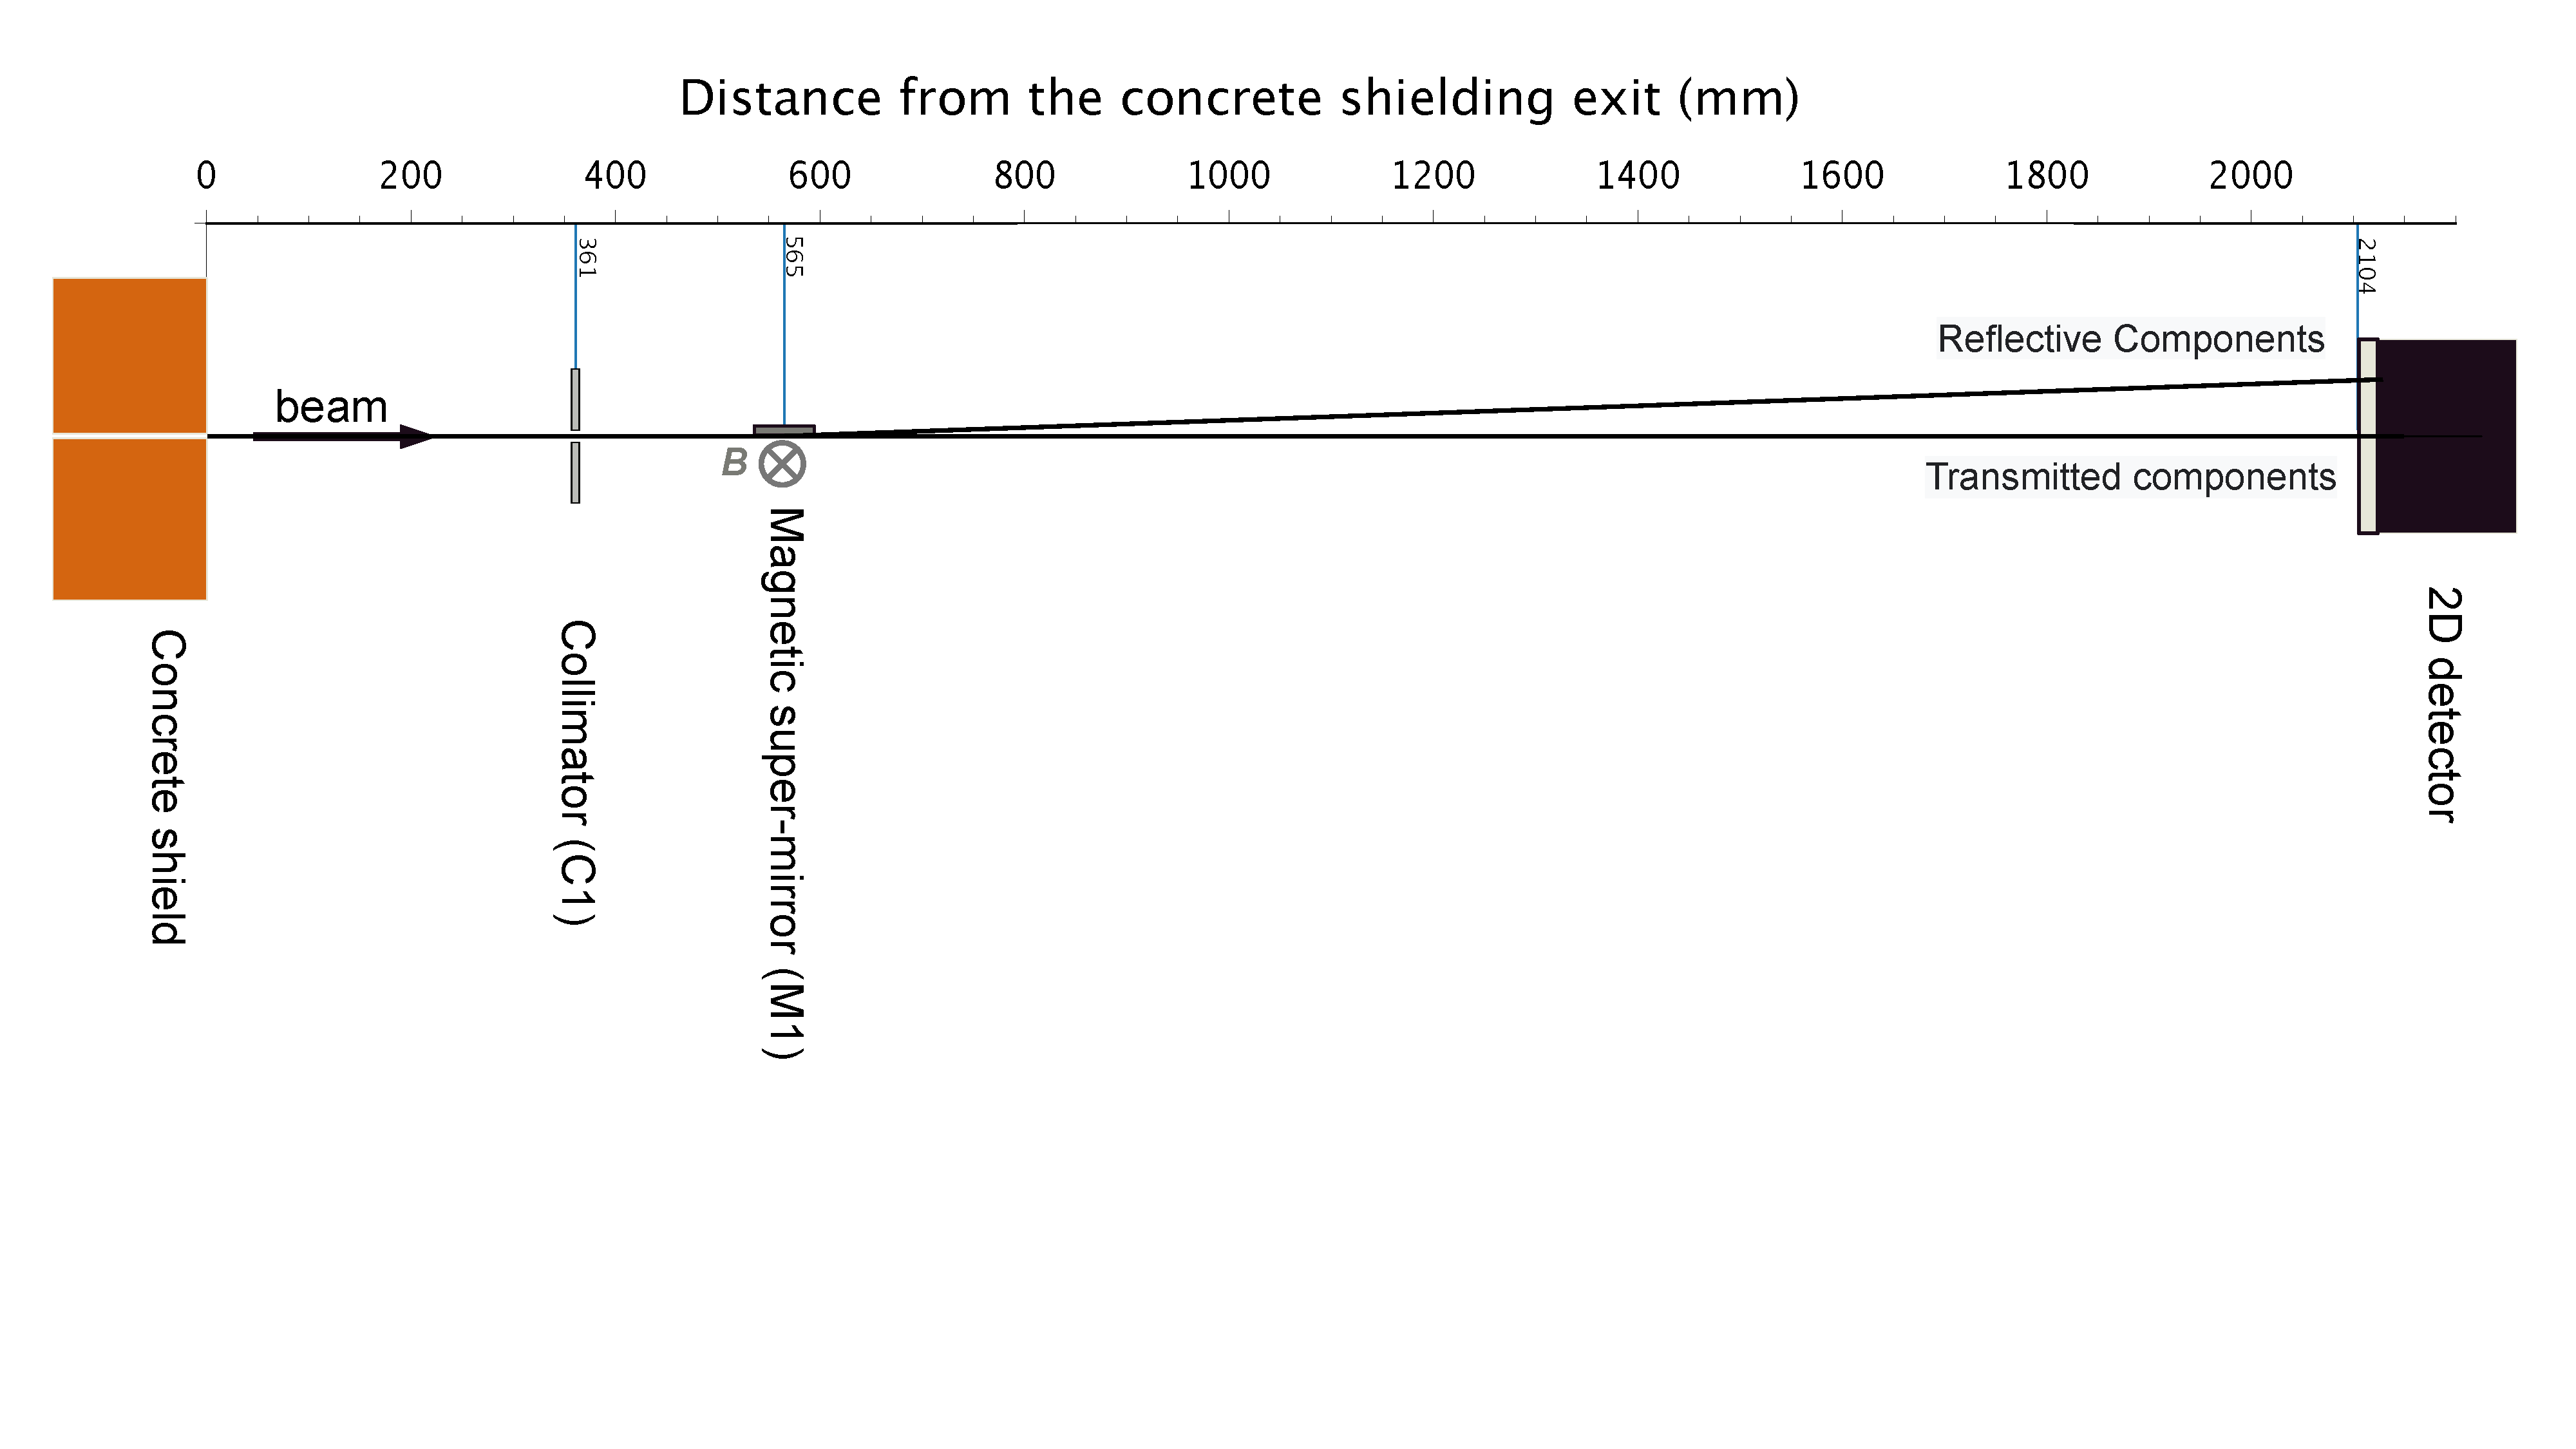
\includegraphics[width=85mm]{BL05_1_2.pdf}
 \includegraphics[width=130mm]{figs/BL05_exp_layout_proc.pdf}
 %\centering
 \caption{a; Setup for cold neutron polarimetry with magnetic supermirror. A neutron beam of $\rm (Vertical)10\,\rm mm\times (Horizontal)0.1\,\rm mm$ is incident on the magnetic supermirror at an angle of incidence of $8.3\,\rm mrad$, and the downstream Position sensitive The reflected and transmitted components were detected by the downstream position sensitive detector (Resistance Photo Multimeter RPMT\cite{RPMT}).
 b; Setup for cold neutron reflectivity measurement with sample. The cold neutron beam was incident on the magnetic supermirror at $10\,\rm mrad$, and the reflected beam was collimated to $\rm (Vertical)10\,\rm mm\times(\rm Horizontal)0.1\,\rm mm$ (Vertical), and then collimated to $12\,\rm mrad$. The sample (iron thin film) was incident at an angle of incidence of $12\,\rm mrad$, and both the reflected and transmitted components were detected by the downstream RPMT. A direct measurement without a sample was performed to measure the incident intensity on the sample, and the reflectance due to the iron film was derived (Fig.\ref{R}).

 }
 \label{setup}
\end{figure}


% \begin{figure}[tbh]
% %  \begin{minipage}{0.5\columnwidth}
%  \centering
% %  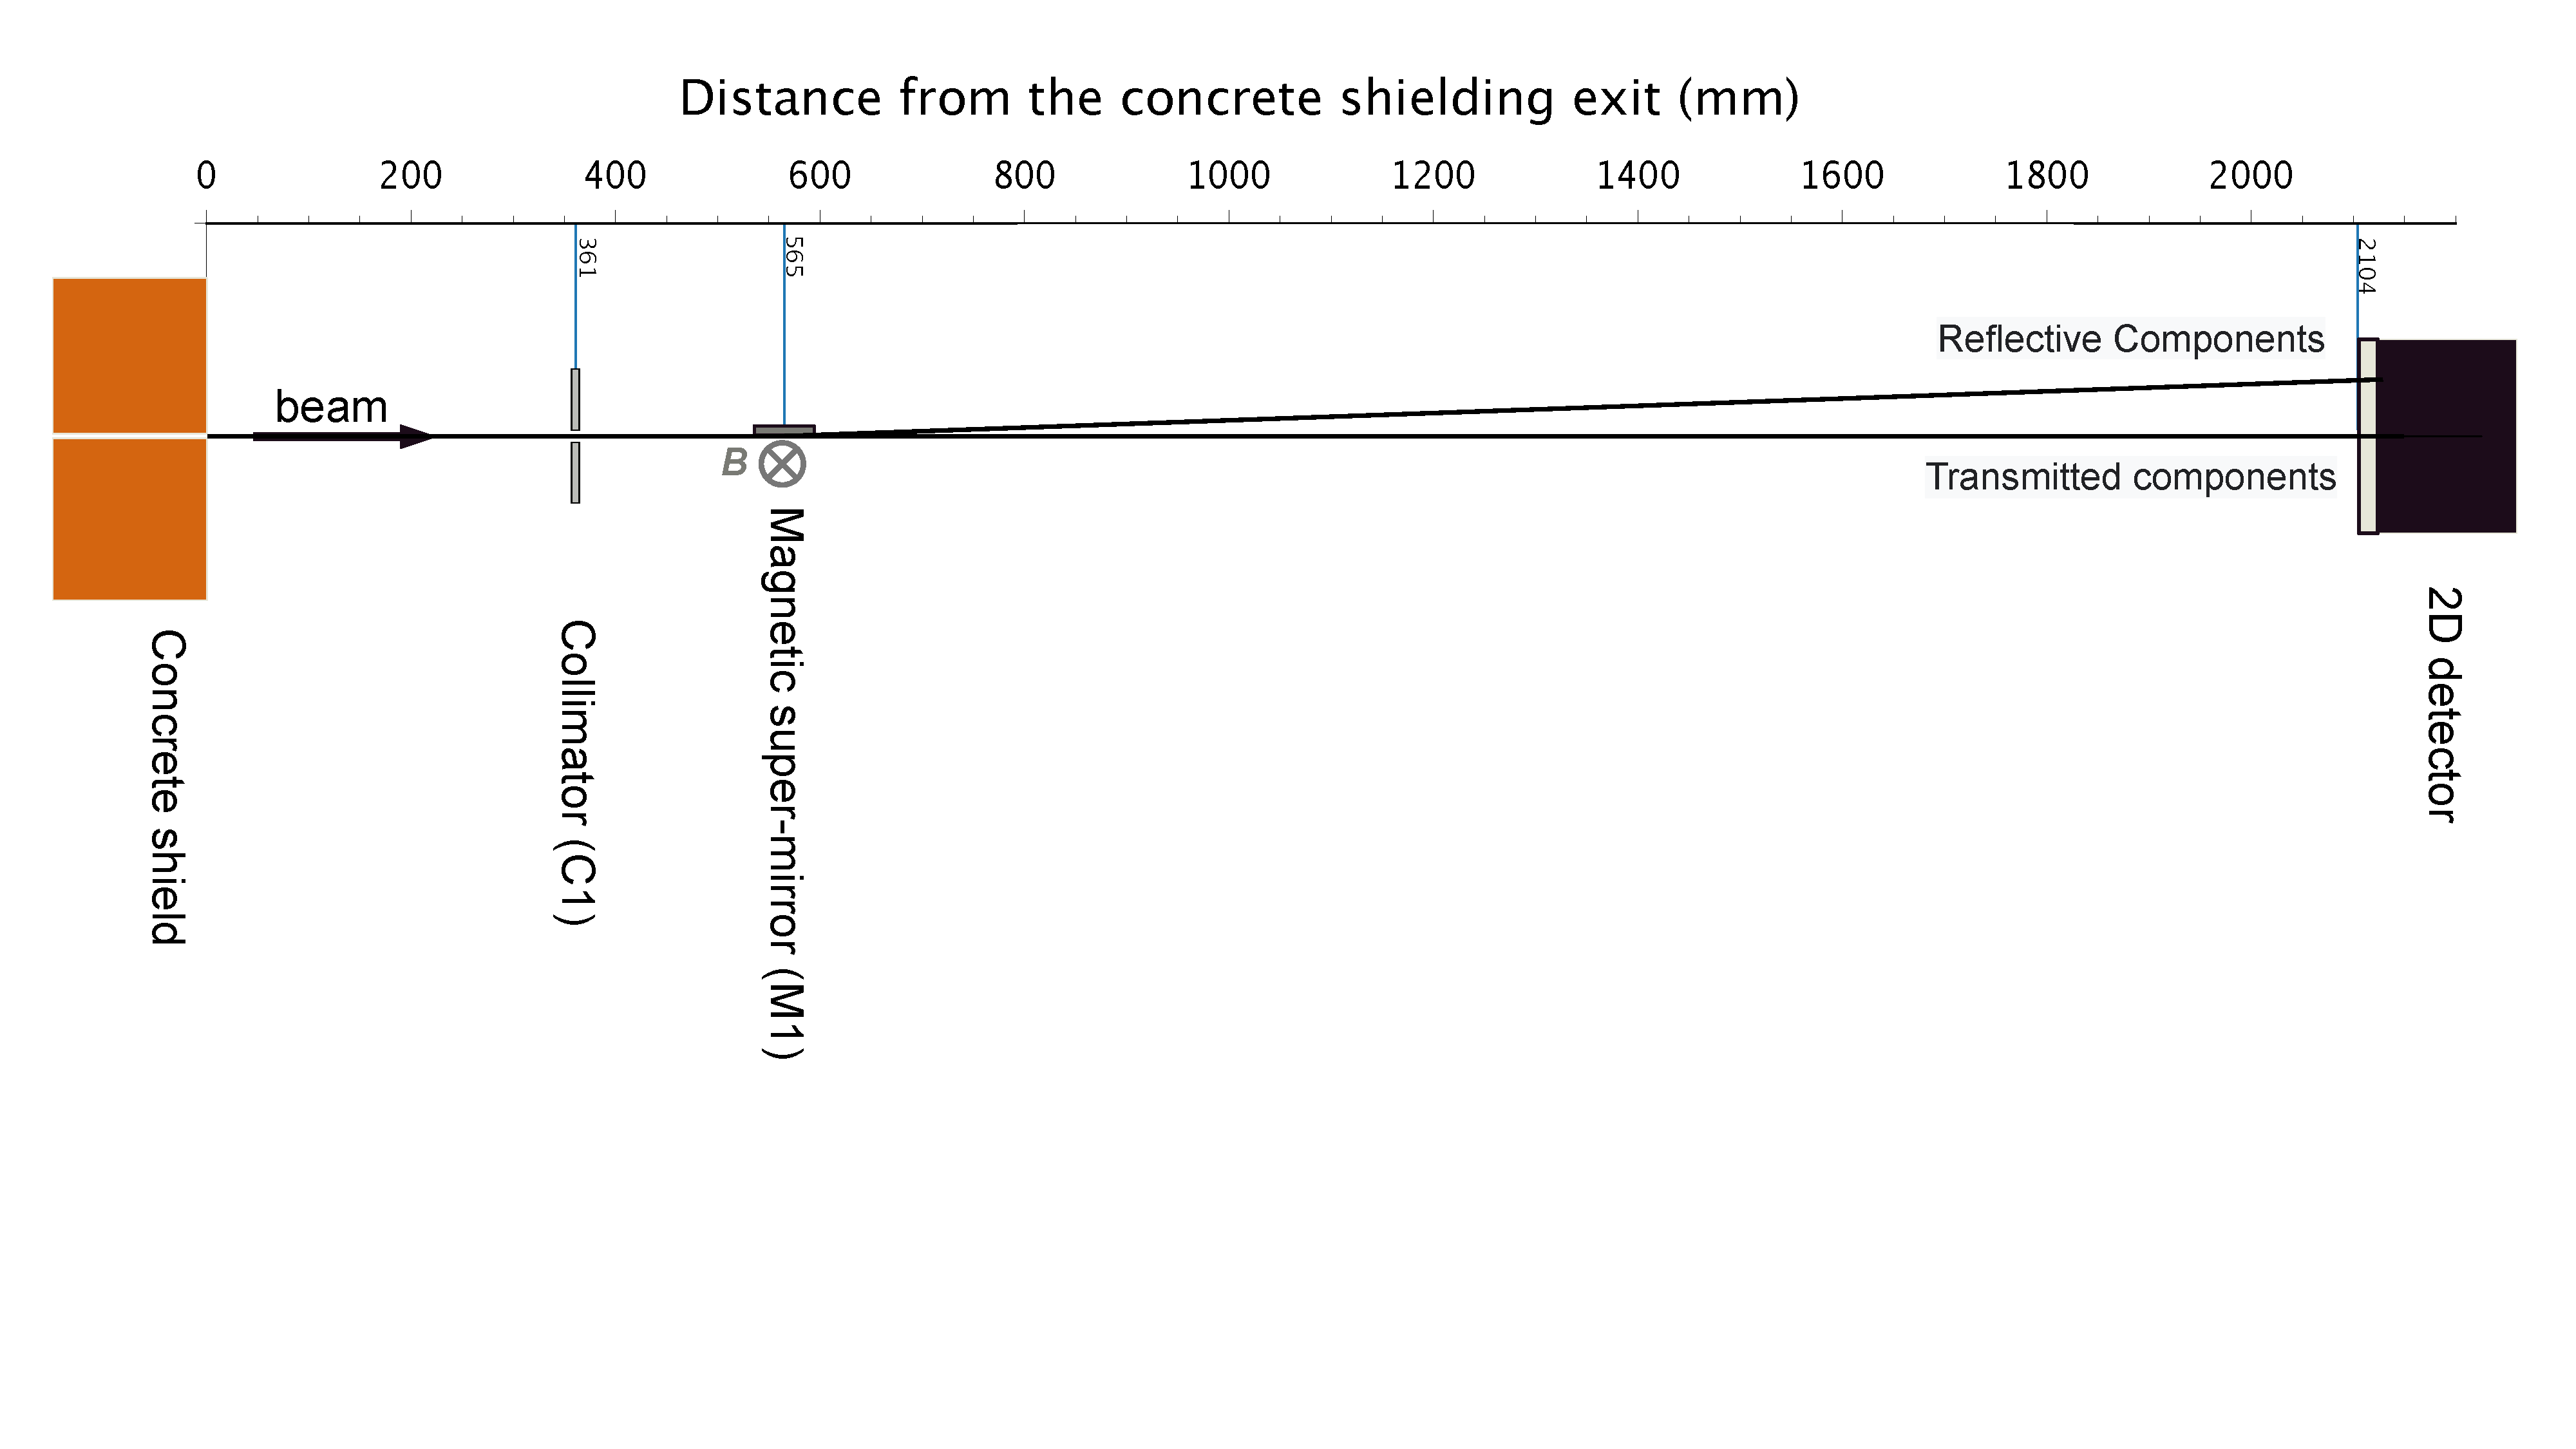
\includegraphics[width=85mm]{BL05_1_2.pdf}
%  \includegraphics[width=130mm]{figs/BL05_exp_layout_proc.pdf}
%  %\centering
%  \caption{a;磁気スーパーミラーによる冷中性子の偏極度測定のセットアップ。$\rm (Vertical)10\,\rm mm\times (Horizontal)0.1\,\rm mm$の中性子ビームを$8.3\,\rm mrad$の入射角で磁気スーパーミラーに入射し、下流のPosition sensitive detector(Resistance Photo Multimeter RPMT\cite{RPMT}) で反射成分および透過成分を検出した。
%  b;試料による冷中性子反射率測定のセットアップ。冷中性子ビームを磁気スーパーミラーに対して$10\,\rm mrad$で入射させ、反射したビームを、$\rm (Vertical)10\,\rm mm\times(\rm Horizontal)0.1\,\rm mm$(縦)にコリメートし、$12\,\rm mrad$の入射角で試料(鉄薄膜)に入射し、下流 の RPMTで反射成分と透過成分の両方を検出した。試料への入射強度を測定するために試料を置かないダイレクト測定を行い、鉄薄膜による反射率を導出した(Fig.\ref{R})。

%  }
%  \label{setup}
% \end{figure}

\begin{figure}[tbh]
 \centering
 \includegraphics[width=130mm]%{base.pdf}%
 {0112_pol.pdf}
 \caption{ (a) Basic principle of the polarizing supermirror. Polarized neutron reflectivity profile of the polarizing supermirror. $R_+$ and $R_-$: Reflectivities for spin-up and -down neutrons. P: Polarization, qz: momentum transfer, $\alpha_i $: incident angle, $\lambda$: neutron wavelength.
 H. Hiraka et al, Hamon, \textbf{28} No.3 144 (2016)[2a,2b]}
 \label{q_pol_temp}
\end{figure}

\subsection{measuring beam polarization}\label{sec:beam-pol}

In the setup of Fig. \ref{setup}a, the magnetic supermirror measured the reflectivity of the mirror. With an unpolarized beam incident, the measured neutron intensity is shown in Fig. \ref{3graph}(a), the reflectivity $R_M$ is shown in Fig. \ref{3graph}(b), and the polarization superposition of the neutron beam by the magnetic super mirror is shown in Fig. \ref{3graph}(c). For the fitting of the reflectivity, $q_c = 0.217 \,\rm nm^{-1},\,m_1=5,\,\alpha=0.2,\,W=0.003$ was fixed and the fitting parameters were $R_0,\,W',\,q_{c,2}$. The fixed values are \cite{KUR}typical values of the magnetic supermirror with $m_1=5$ fabricated at the KURNS IBS. The fitting
The result was $R_0=0.9923(9),\,W'=0.152(2),\,q_{c,2}=0.140(2)$, and this value was substituted into the equations (\ref{RM2},\ref{RM3}) to determine the polarization.

% \subsection{ビームの偏極度測定}\label{sec:beam-pol}

% 図\ref{setup}a のセットアップで磁気スーパーはミラーの反射率を測定した。非偏極ビームを入射した場合、測定された中性子強度を図\ref{3graph}(a)に、反射率$R_M$を図\ref{3graph}(b)に、磁気スーパーミラーによる中性子ビームの偏極度を図\ref{3graph}(c)に示した。反射率のフィッティングでは、$q_c = 0.217 \,\rm nm^{-1},\,m_1=5,\,\alpha=0.2,\,W=0.003$ を固定し、fittingパラメータを$R_0,\,W',\,q_{c,2}$とした。固定した値は、KURNSのIBSで製作された$m_1=5$の磁気スーパーミラーのtypicalな値を用いた\cite{KUR}。フィッティングの
% 結果、$R_0=0.9923(9),\,W'=0.152(2),\,q_{c,2}=0.140(2)$となり、この値を式(\ref{RM2},\ref{RM3})に代入して、偏極度を決定した。

 \begin{figure}[tbh]
 %\centering
 
\includegraphics[width=100mm]{0112_3graph.pdf}
 \centering
 \caption{(a):Position dependence of the neutron intensity detected by the RPMT in Figure \ref{setup}. A histogram of neutron intensities integrated over a range of $30\,\rm mm$ in the vertical direction is packed. The integrated intensity in the range enclosed by the bink line is the reflected intensity $I_R$, and the integrated intensity in the range enclosed by the black line is the transmitted intensity $I_T$, defined as $R_M=\frac{I_R}{I_R+I_T}$. (b):Wavelength dependence of $R_M=$. Equation (\ref{RM})
 %(\ref{RM2},\ref{RM2,1},\ref{RM3},\ref{RM3,1})
 Fitted with (c):Wavelength dependence of the polarization $P=(R_{+}-R_{-})/(R_{+}+R_{-})$. We obtained $P$ from $R_{+},R_{-}$ in the fit results of Figure \ref{3graph}(b).
 }
 \label{3graph}
 \end{figure}
 
%  \begin{figure}[tbh]
%  %\centering
%  
\includegraphics[width=170mm]{0112_3graph.pdf}
%  \centering
%  \caption{(a):図\ref{setup}においてRPMTによって検出された中性子強度の位置依存性。縦方向に$30\,\rm mm$の範囲で積算した中性子強度をヒストグラムに詰めた。ビンクの直線で囲まれた範囲の積分強度を反射強度$I_R$、黒の直線で囲まれたはにの積分強度を透過強度$I_T$として、$R_M=\frac{I_R}{I_R+I_T}$と定義した。(b):$R_M=$の波長依存性。式(\ref{RM})
%  %(\ref{RM2},\ref{RM2,1},\ref{RM3},\ref{RM3,1})
%  でフィットした。(c):偏極度$P=(R_{+}-R_{-})/(R_{+}+R_{-})$の波長依存性。図\ref{3graph}(b)のフィット結果の$R_{+},R_{-}$から$P$を求めた。
%  %図\ref{setup}a のセットアップで測定した、中性子強度の横方向の位置分布を図\ref{mirror_x}に示した。反射成分の中性子強度$I_R$、透過成分の中性子強度$I_T$を用いて、$R_M=\frac{I_M}{I_M+I_T}$と定義した。
%  }
%  \label{3graph}
%  \end{figure}

\subsection{Reflectance measurement of iron thin film sample}\label{sec:sample}
%Next, from the relationship between $q$ and the reflectivity
In order to determine the magnitude of the neutron potential in the sample based on the relationship between $q$ and the reflectivity, cold neutron reflectivity measurements were performed with the setup shown in Fig.\ref{setup}b.
In addition to the above setup (Fig.\ref{setup_pol}), a spin flipper, an electromagnet, and a sample were set up. (Fig.\ref{spline})
The polarized cold neutron beam obtained in the \ref{{sec:beam-pol}} chapter was injected into the sample magnetized by the electromagnet by selecting the spin state by turning on and off the spin flipper, and the reflectivity was measured.

The measured neutron intensity is shown in Fig. \ref{mirror_x} and the reflectivity $R^s_{\pm}$ is shown in Fig. \ref{R}.
For the fitting of the reflectance, the thickness of the iron film, $d=89.066\,\rm nm$, determined from the X-ray reflectivity measurement, was fixed and $V_{\rm Fe},\,B$ were globalfit as common parameters for the experimental results of $R^s_{+},R^s_{-}$. As a result, $V_{\rm Fe}=186(1)\,\rm neV,\,B=2.02(1)\,\rm T$, and the potentials $V_{\rm Fe,-},\,V_{\rm Fe,+}$ are $V_{\rm Fe,-},\,V_{\rm Fe,+}$ when the neutron spin is parallel or antiparallel to the magnetized direction of the iron film, respectively. $V_{Fe,-}=64(1)\,\rm neV,\,V_{\rm Fe,+}=308(1)\,\rm neV$, respectively. Therefore, the saturation magnetization of the fabricated sample is close to that of bulk iron at $\sim 2\,\rm T$ and %$64\,\rm neV<E_{en}<308\,\rm neV$.
It was confirmed that polarization analysis is possible in the energy range from $64\,\rm neV$ to $308\,\rm neV$.

% \subsection{鉄薄膜試料の反射率測定}\label{sec:sample}
% %次に、$q$と反射率の関係から、
% 中性子が試料中で感じるポテンシャルの大きさを決定するために、図\ref{setup}b のセットアップで、冷中性子反射率測定を行なった。
% %上記のセットアップ(Fig.\ref{setup_pol})に加え、スピンフリッパー、電磁石、試料をセットした。(Fig.\ref{spline})のように
% \ref{{sec:beam-pol}}章で得た偏極度の冷中性子ビームをスピンフリッパーのON, OFFによってスピン状態を選択し、電磁石で磁化させた試料に入射させ、反射率を測定した。

% 測定された中性子強度を図\ref{mirror_x}に、反射率$R^s_{\pm}$を図\ref{R}に示した。
% 反射率のフィッティングでは、X線反射率測定から決定した鉄薄膜の厚さ$d=89.066\,\rm nm$を固定し$V_{\rm Fe},\,B$を、$R^s_{+},R^s_{-}$の実験結果に対して共通のパラメータとしてglobalfitを行なった。その結果、$V_{\rm Fe}=186(1)\,\rm neV,\,B=2.02(1)\,\rm T$となり、中性子のスピンが鉄薄膜の磁化した方向と平行、反平行な場合のポテンシャル$V_{\rm Fe,-},\,V_{\rm Fe,+}$は、それぞれ$V_{\rm Fe,-}=64(1)\,\rm neV,\,V_{\rm Fe,+}=308(1)\,\rm neV$となった。よって、作製した試料の飽和磁化がバルクの鉄に近い$\sim 2\,\rm T$の飽和磁化を持ち、%$64\,\rm neV<E_{en}<308\,\rm neV$
% $64\,\rm neV$から$308\,\rm neV$のエネルギー領域で偏極解析が可能であることが確認された。



% 試料による中性子の反射率は、厚さ(数十 nm)の鉄薄膜に対して、基板の厚さを十分大きいと仮定した時の理論式により、次のように表すことができる。\\
% $E>V_{\rm Fe}$の時、
% \begin {align}
% R=\frac{(k_0k_1-k_1k_2)^2\cos^2(k_1d)+(k_0k_2-k_1^2)^2\sin^2 (k_1d)}{(k_0k_1+k_1k_2)^2\cos^2(k_1d)+(k_0k_2+k_1^2)^2\sin^2 (k_1d)}
% \end{align}
% $V_{\rm Fe}>E>V_{\rm Si}$の時、
% \begin {align}
% R=\frac{(\alpha k_0-\alpha k_2)^2\cosh^2(\alpha d)+(k_0k_2+\alpha^2)^2\sinh^2 (\alpha d)}{(\alpha k_0+\alpha k_2)^2\cosh^2(\alpha d)+(\alpha^2-k_0k_2)^2\sinh^2 (\alpha d)}
% \end{align}
% $E<V_{\rm Si}$の時、
% \begin {align}
% R=1
% \end{align}
% ここで、$k_0=\frac {\sqrt{2m_nE} }{\hbar},\,k_1=\frac {\sqrt{2m(E-V)} }{\hbar},\,k_2=\frac {\sqrt{2m(E-V_{\rm Si})} }{\hbar},\,\alpha=\frac {\sqrt{2m(V-E)} }{\hbar}\,$はそれぞれ真空中、鉄薄膜中、Si基板中の中性子の波数、$m_n$は中性子の質量、$V$は中性子が感じるポテンシャル、$V_{\rm Si}$はSiのフェルミポテンシャル、$d$は鉄薄膜の厚みを表す。中性子が感じるポテンシャル$V=V_{\rm Fe}\pm \mu_n B$は、鉄のフェルミポテンシャル$V_{\rm Fe}$、中性子の磁気モーメント$\mu_n$、鉄内部の磁束密度$\boldsymbol B$によって表される。
% 上記の式で、X線反射率測定から決定した鉄薄膜の厚さ$d=89.066\,\rm nm$を固定し$V_{\rm Fe},\,B$ をパラメータとして実験結果をフィッティングすると、$V_{\rm Fe}=186(1)\,\rm neV,\,B=2.02(1)\,\rm T$となり、中性子のスピンが鉄薄膜の磁化した方向と平行、反平行な場合のポテンシャル$V_{\rm Fe,-},\,V_{\rm Fe,+}$は、それぞれ$V_{\rm Fe,-}=64(1)\,\rm neV,\,V_{\rm Fe,+}=308(1)\,\rm neV$となった。よって、作製した試料の飽和磁化がバルクの鉄に近い$\sim 2\,\rm T$の飽和磁化を持ち、%$64\,\rm neV<E_{en}<308\,\rm neV$
% $64\,\rm neV$から$308\,\rm neV$のエネルギー領域で偏極解析が可能であることが確認された。


\begin{figure}[tbh].
 %\centering
 \begin{minipage}[t]{0.45\columnwidth}
 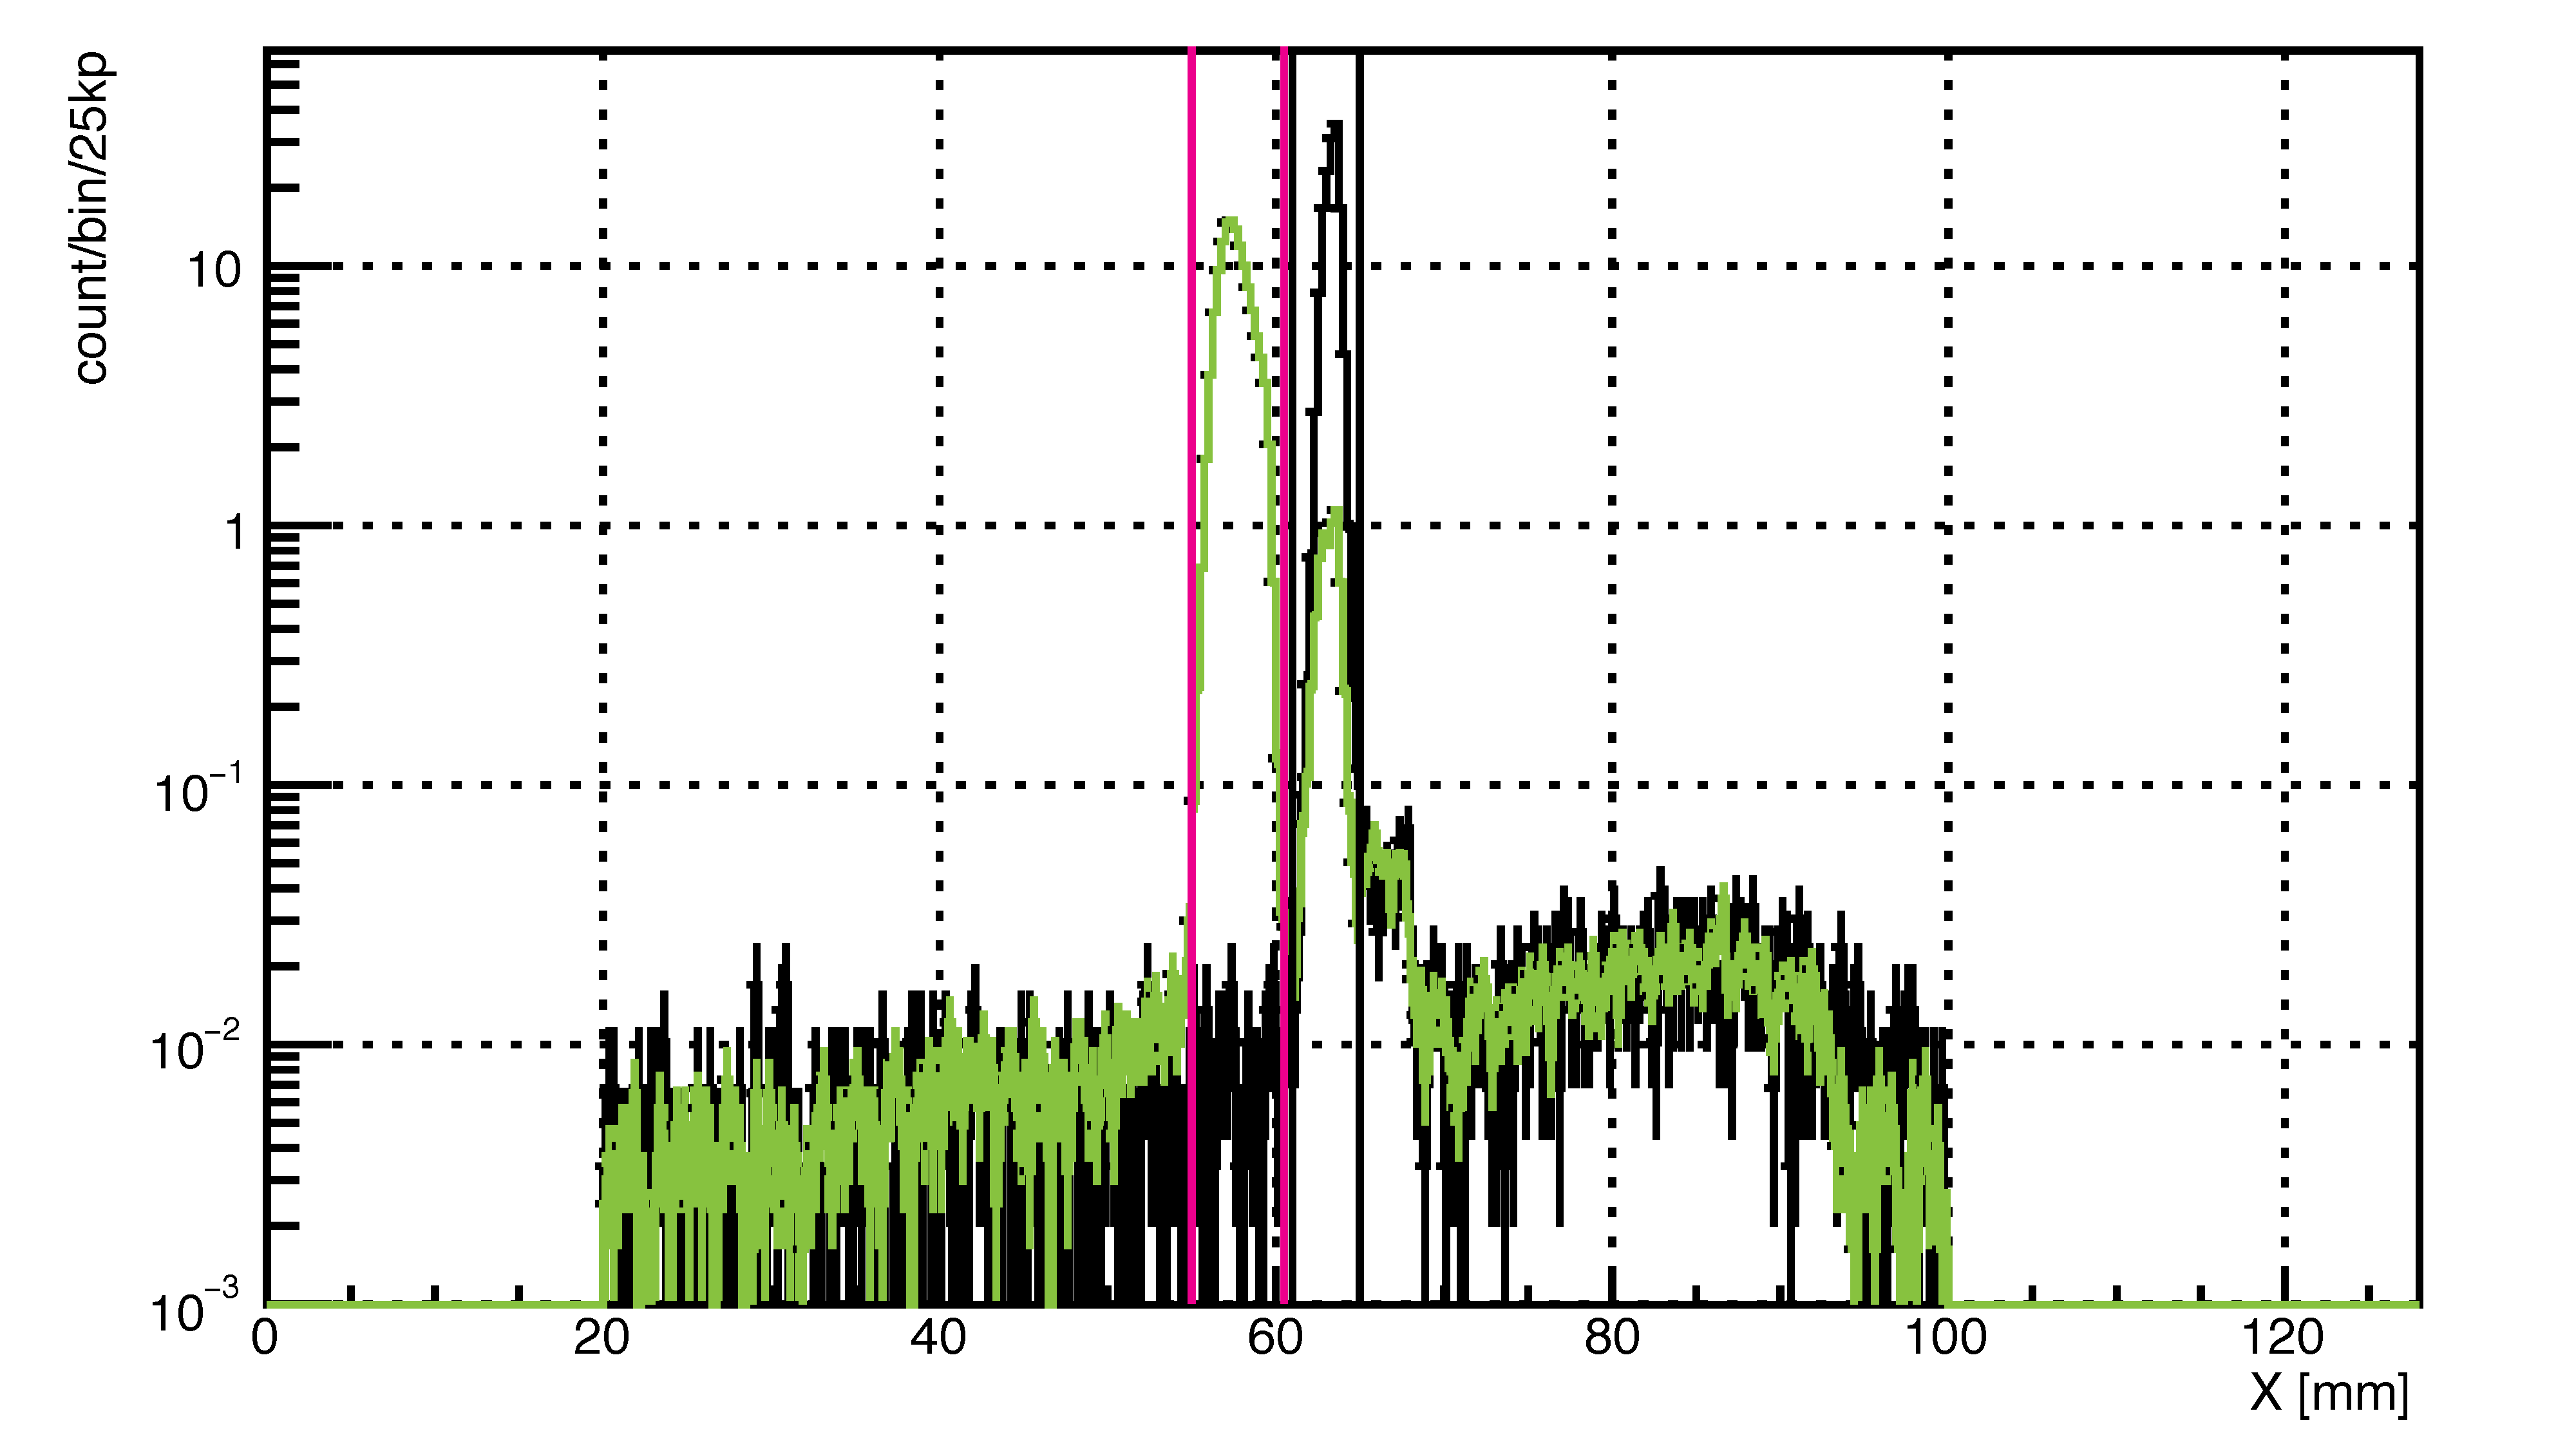
\includegraphics[width=75mm]{0110_X_I_M1.pdf}
 \centering
 \caption{position dependence of the neutron intensity detected by the RPMT in Figure \ref{setup_R}. Histogram of neutron intensities integrated over a range of $30\,\rm mm$ in the vertical direction. The histogram (Green) shows the neutron intensity when neutrons are incident on the sample, and the histogram (Black) shows the neutron intensity during direct measurement without placing the sample. The integrated intensity of the histogram (Green) in the range enclosed by the bink lines is defined as the reflection intensity $I^s_{ R}$, and the integrated intensity of the histogram (Black) enclosed by the black lines is defined as the incident intensity $I^s_{\rm in}$.}
 \label{mirror_x}
 \end{minipage}
 \hspace{0.1\columnwidth}
 %\centering
 \begin{minipage}[t]{0.45\columnwidth}
  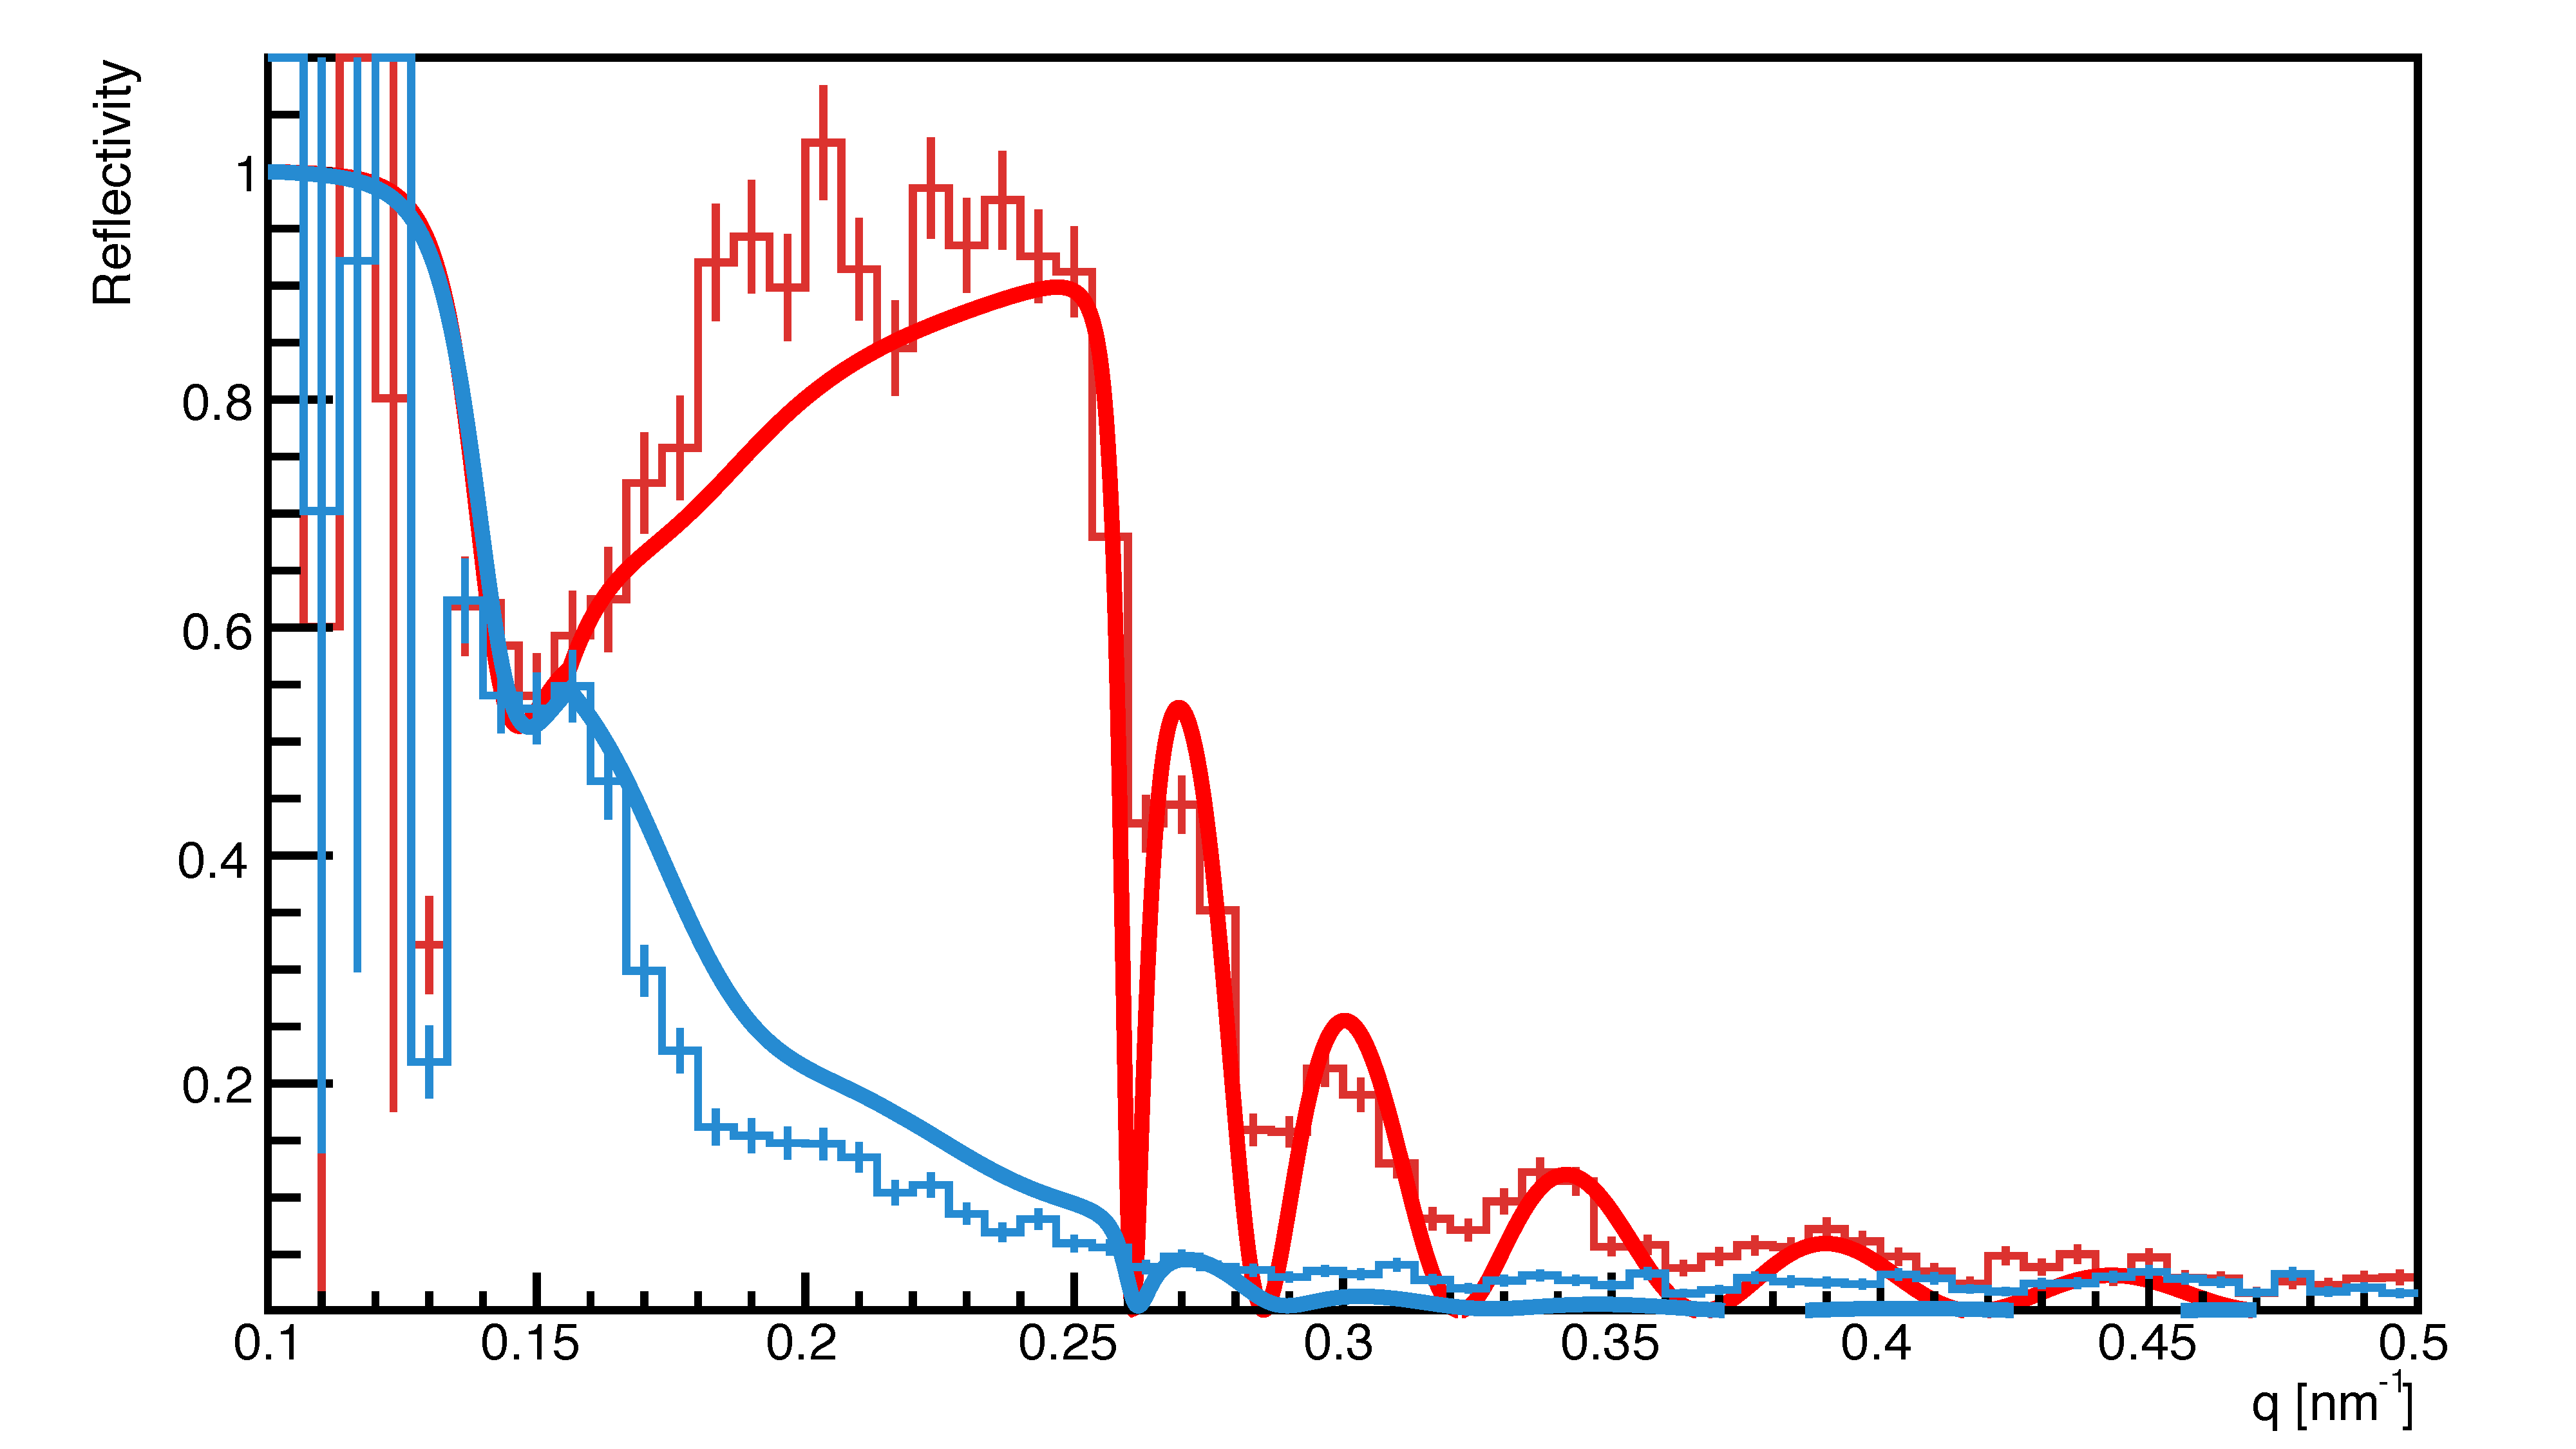
\includegraphics[width=70mm]{0110_global.pdf}
  %{reflectivity.pdf}
  \centering
  \caption{Histogram shows the momentum transfer dependence of the spin(+)(red) and spin(-)(blue) neutron reflectivity on the sample, the curve is a function of the reflectivity fitted with \ref{Rs}.
  }
  \label{R}
 \end{minipage}
\end{figure}

\section{Conclusions and Outlook}
TUCAN aims to measure nEDM with an accuracy of $10^{-27}\rm e\cdot cm$, an order of magnitude improvement over the current highest search sensitivity. nEDM measurements require measurement of neutron polarization. In order to obtain a large energy region for polarization analysis with SSA, the iron thin film needs to have a large saturation magnetization. In addition, it is desirable to operate the SSA with as small an applied magnetic field as possible in order not to affect other devices and to increase the degree of freedom in design. Therefore, we fabricated iron thin films and evaluated their magnetic properties. In addition to the Al-based iron films developed in the previous study \cite{SSA}, we have also fabricated Si-based iron films by performing VSM measurements on the Al-based iron films and Si-based polarization analysis films, and cold neutron reflectivity measurements on the Si-based iron films. VSM measurements were carried out for each sample, and cold neutron reflectivity measurements were carried out for the Si-based iron film, confirming that it meets our target performance of iron thin films.
The VSM measurements confirmed that the iron film with Al substrate saturates at ($\sim 15\rm\,mT$) and the iron film with Si substrate saturates at ($\sim 5\rm\,mT$), which is smaller than the applied magnetic field ($\sim 50\rm\,mT$) in the previous study \cite{SSA}. In the neutron reflectivity measurement, we found that the Neutron reflectivity measurements show that the iron film saturates at an applied field of $8.13\,\rm mT$.
%$64\,\rm neV<E_{en}<
It was confirmed that polarization analysis in the energy region from $64$--$308\,\rm neV$ is possible.
These measurements confirm that the introduction of iron thin films on Si substrates into nEDM search experiments is promising.
In the spring of 2022, we plan to conduct reflectivity measurements using UCN for more accurate evaluation of iron thin films.





% \begin{figure}[tbh]
%  %\centering
%  \begin{minipage}[t]{0.45\columnwidth}
%  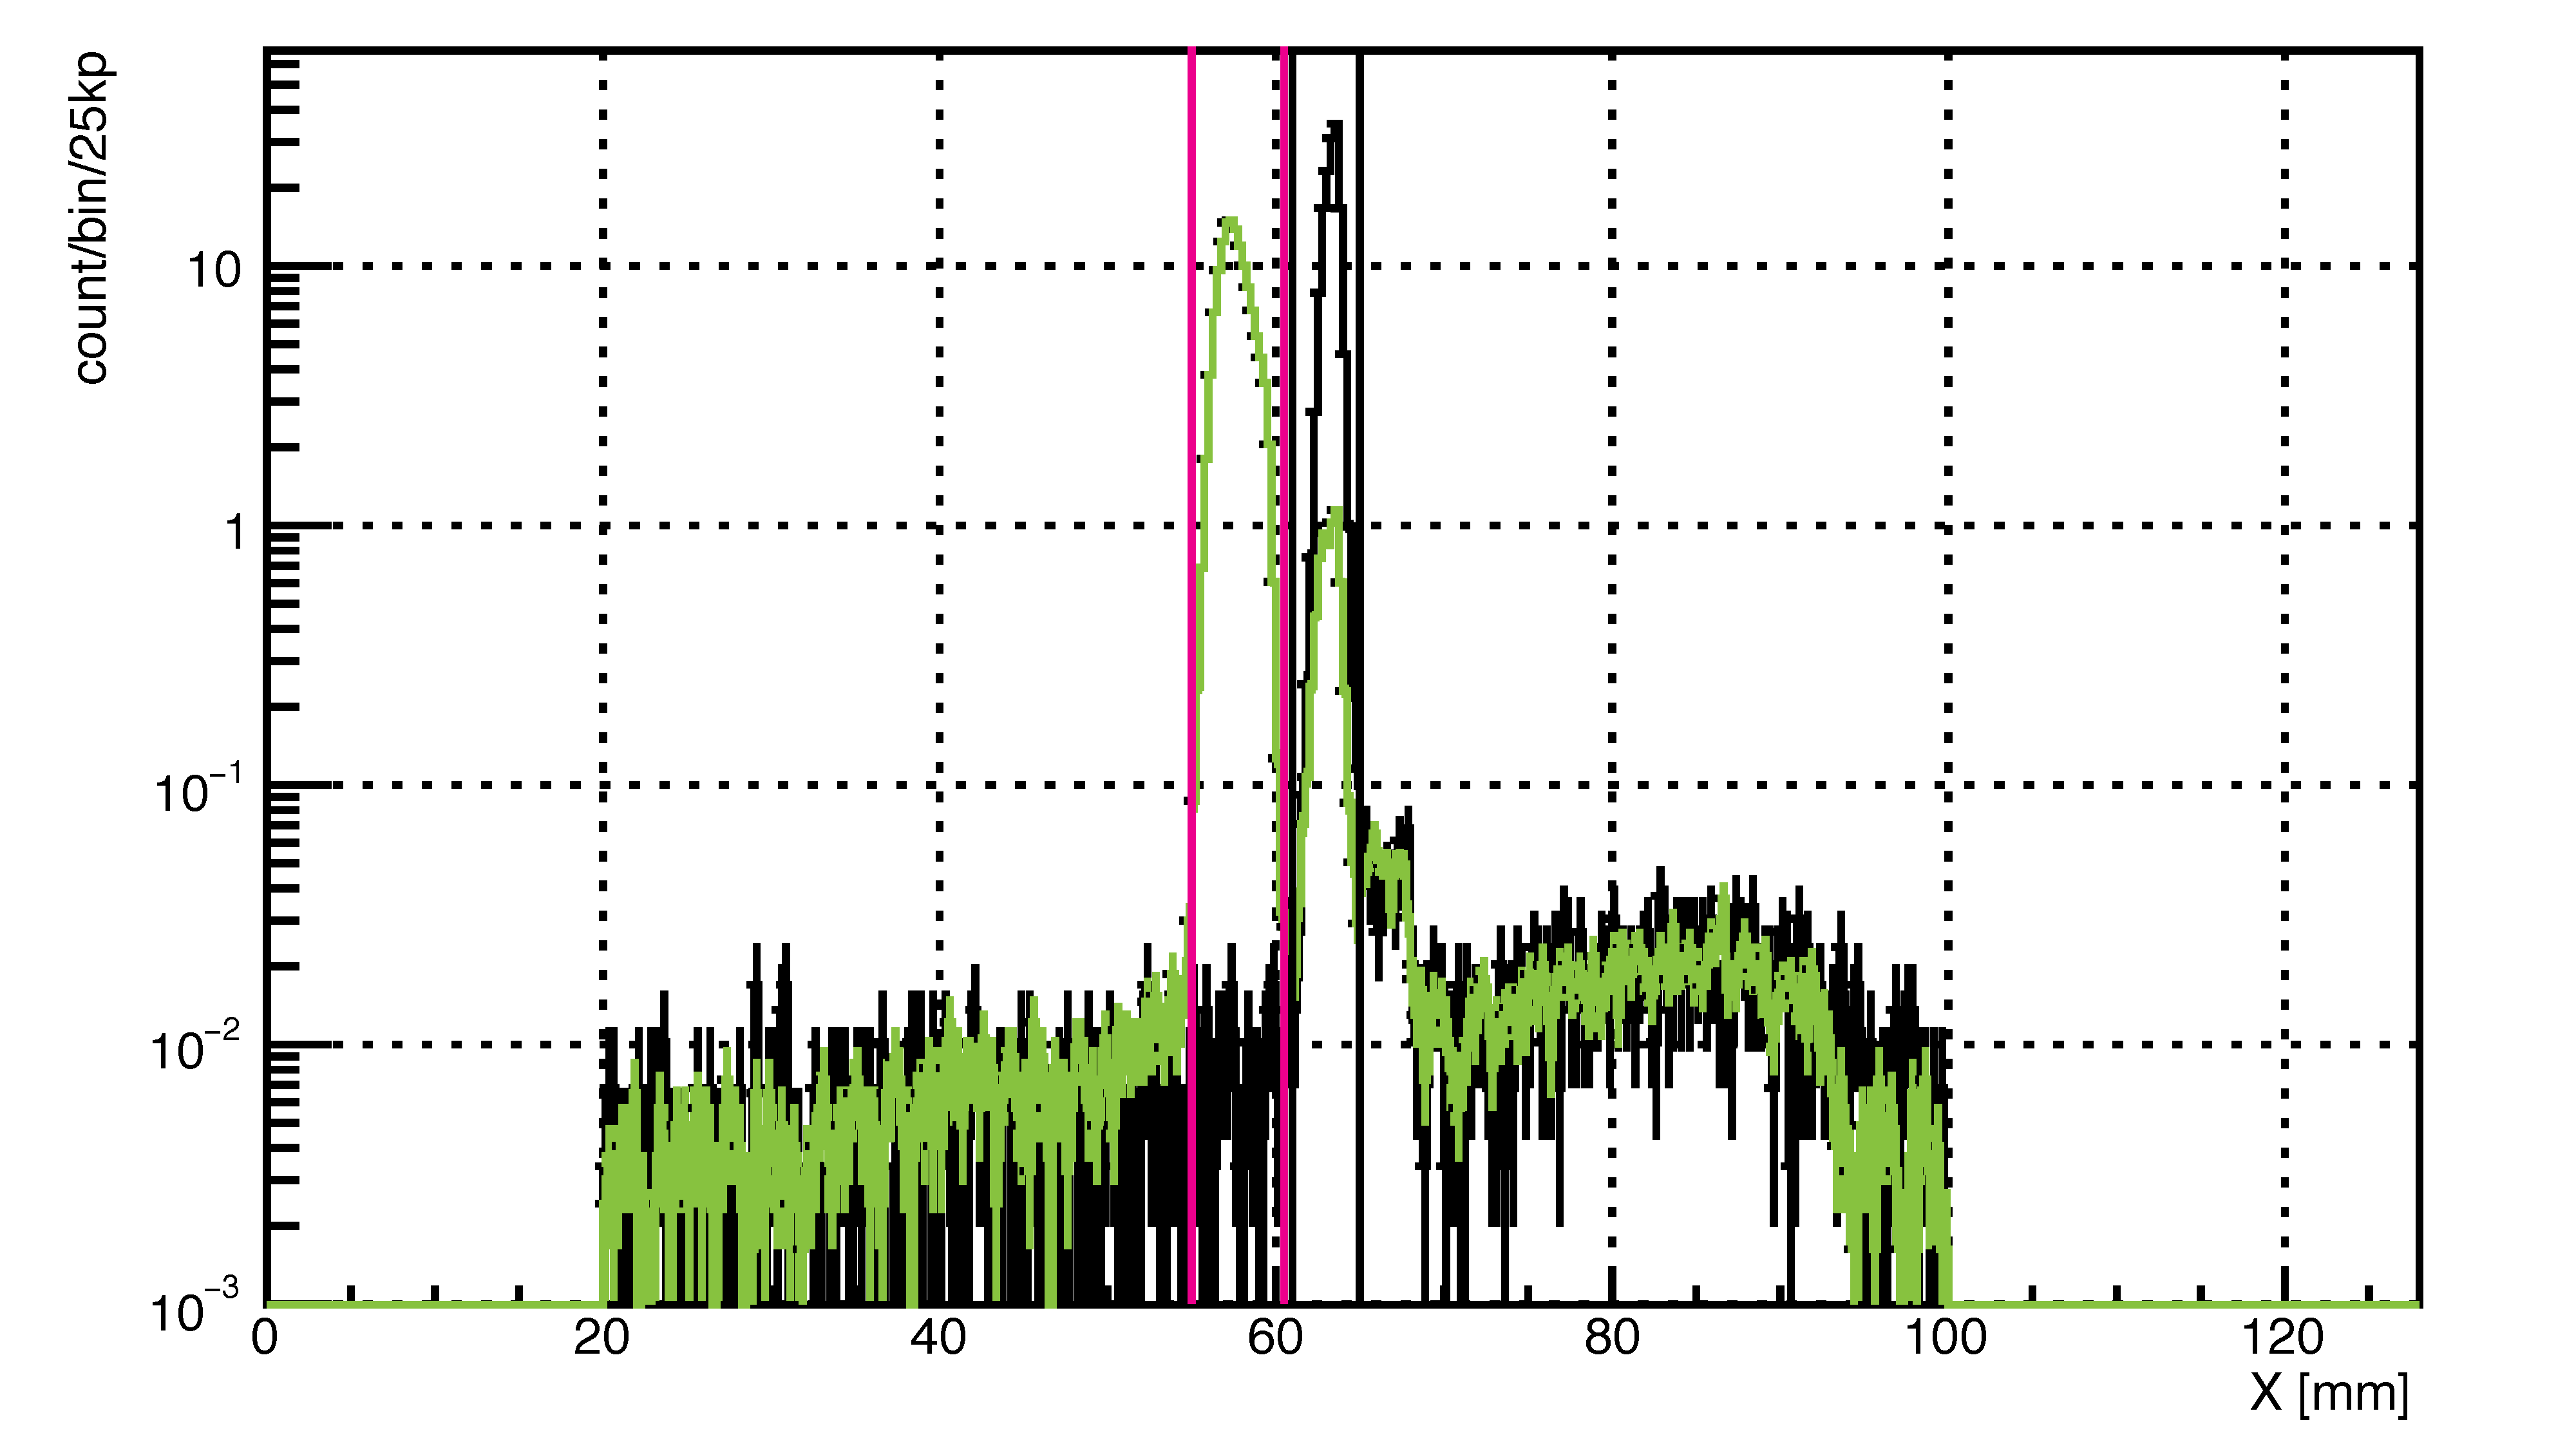
\includegraphics[width=75mm]{0110_X_I_M1.pdf}
%  \centering
%  \caption{図\ref{setup_R}においてRPMTによって検出された中性子強度の位置依存性。縦方向に$30\,\rm mm$の範囲で積算した中性子強度をヒストグラムに詰めた。ヒストグラム(Green)は中性子を試料に入射させた際の中性子強度、ヒストグラム(Black)は試料を置かずに測定するダイレクト測定の際の中性子強度。ビンクの直線で囲まれた範囲のヒストグラム(Green)の積分強度を反射強度$I^s_{ R}$、黒の直線で囲まれたヒストグラム(Black)の積分強度を入射強度$I^s_{\rm in}$と定義した。}
%  \label{mirror_x}
%  \end{minipage}
%  \hspace{0.1\columnwidth}
%  %\centering
%  \begin{minipage}[t]{0.45\columnwidth}
%   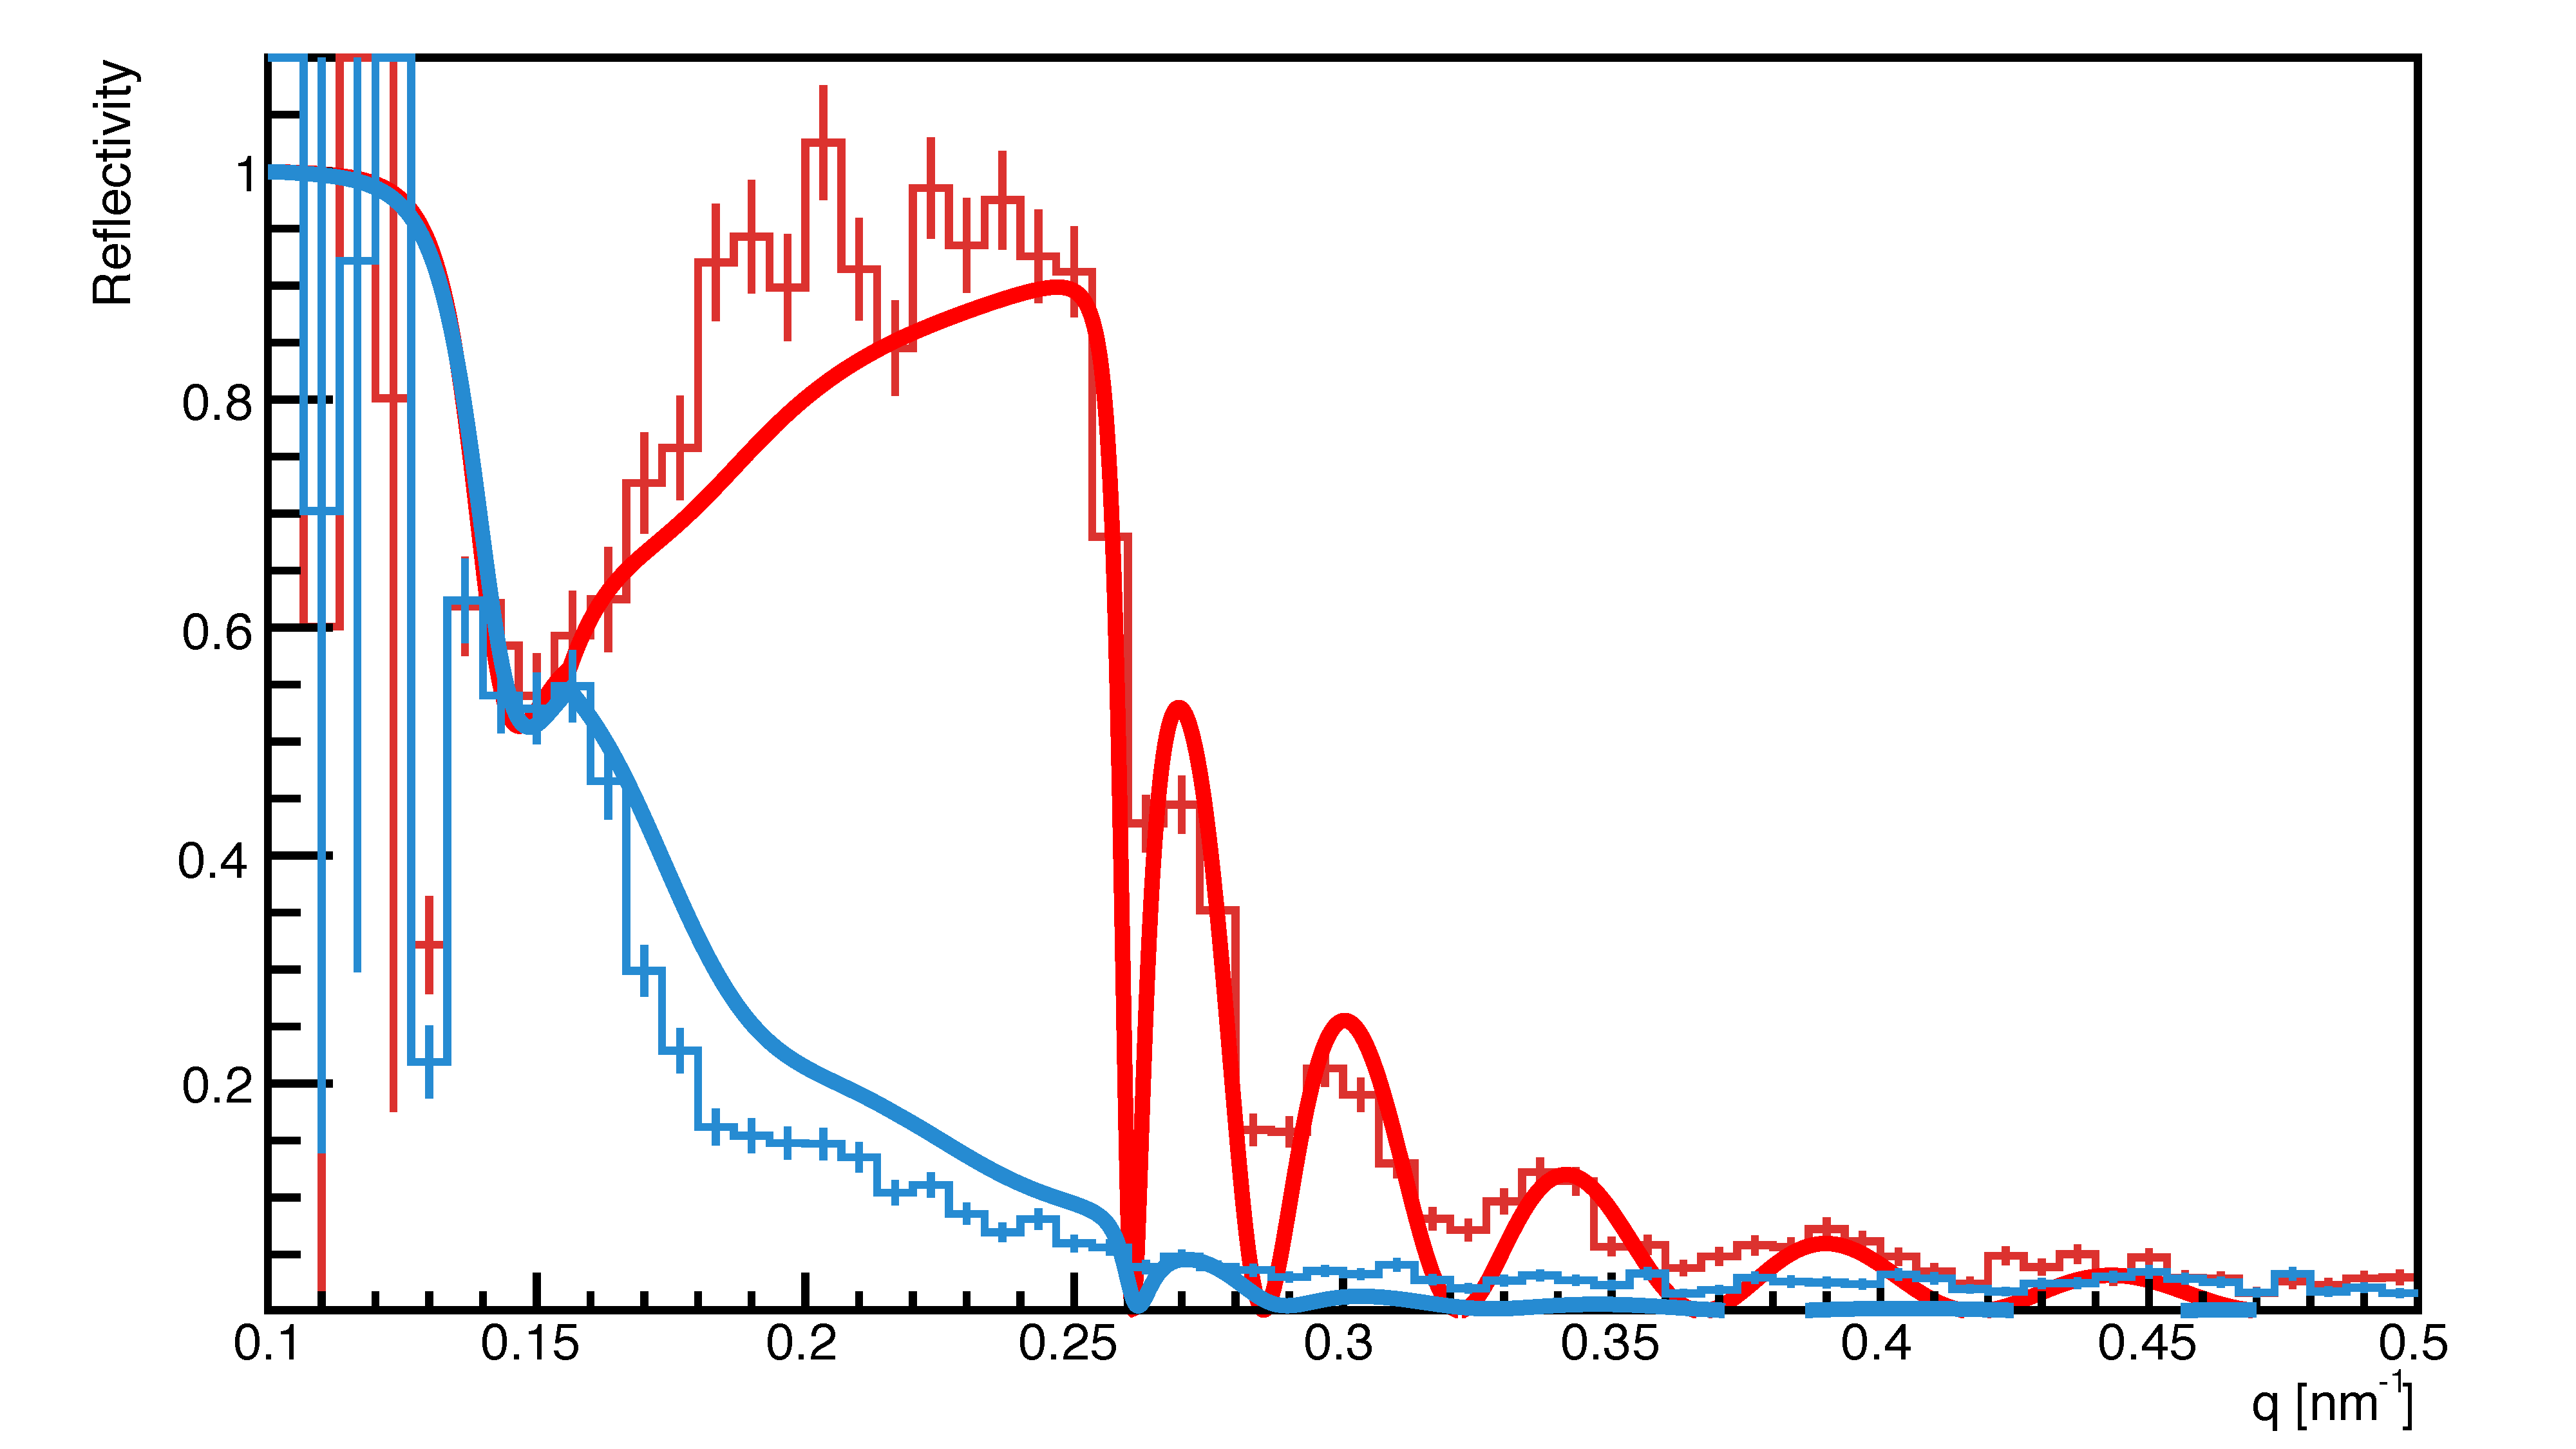
\includegraphics[width=75mm]{0110_global.pdf}
%   %{reflectivity.pdf}
%   \centering
%   \caption{ヒストグラムは試料にによるspin(+)(red),spin(-)(blue)中性子の反射率の運動量移行依存性、曲線は反射率を\ref{Rs}でフィットした関数を表す。
%   %Neutron reflectivity of spin(+)(blue), spin(-)(red) and fitting curve of $\rm Fe$ 90 nm on a silicon substrate.
%   }
%   %, 50 nm (green), 90 nm (purple)}
%   \label{R}
%  \end{minipage}
%  %\figlab{sample}
% \end{figure}

% \section{Conclusions and Outlook}
% TUCANはnEDMを$10^{-27}\rm e\cdot cm$の精度で測定し、現在の最高探索感度を1桁向上させることを目標としている。nEDMを測定するためには、中性子の偏極度を測定する必要がある。偏極度を測定する装置SSAで偏極解析可能なエネルギー領域を大きく取るためには、鉄薄膜がより大きな飽和磁化を持つ必要がある。またSSAは、他装置に影響を与えず、さらに設計の自由度を大きくするため、なるべく小さな印加磁場で動作することが望ましい。そこで、我々は鉄薄膜の製作と磁気特性の評価を行なった。先行研究\cite{SSA}で開発された、Al基板を用いた鉄薄膜に加え、Si基板を用いた鉄薄膜を作製した。Al基板を用いた鉄薄膜、Si基板を用いた偏極解析膜、それぞれの試料に対してVSM測定を行い、Si基板を用いた鉄薄膜に対して冷中性子反射率測定を行うことで、我々が目指している鉄薄膜の性能を満たしていることを確かめた。
% VSM測定によって、Al基板を用いた鉄薄膜が($\sim 15\rm\,mT$)で、Si基板を用いた鉄薄膜が($\sim 5\rm\,mT$)で飽和することが確認され、先行研究\cite{SSA}での印加磁場($\sim 50\rm\,mT$)よりも小さい印加磁場で飽和することがわかった。中性子反射率測定では、鉄薄膜が$8.13\,\rm mT$の印加磁場で
% %$64\,\rm neV<E_{en}<
% $64$から$308\,\rm neV$のエネルギー領域の偏極解析が可能であることが確認された。
% これらの測定により、Si基板を用いた鉄薄膜のnEDM探索実験への導入が有望であることが確かめられた。
% 今後は2022年の春にUCNを用いた反射率測定を行い、より正確な鉄薄膜の評価が計画されている。






\section{Acknowledgements}
\par
This research was supported by JSPS KAKENHI 
Grant Number 18H05230 and 20KK0069.
%Grant-in-Aid for Scientific Research(S) 
%Grants-in-Aid for Scientific Research Fund for the Promotion of Joint International Research (Fostering Joint International Research(B)) 
The neutron experiment at the Materials and Life Science Experimental Facility of the J-PARC was performed under user S-type project of KEK (Proposal No. 2019S03).  The iron thinfilm fabrication work has been carried out under the visiting Researcher’s Program of the Institute for Integrated Radiation and Nuclear Science, Kyoto University.



% You can use this file as a template to prepare your manuscript for JPS Conference Proceedings\cite{cp,jpsj,ptep,instructions,format}.

% Copy \verb|jps-cp.cls| and \verb|cite.sty| onto an arbitrary directory under the texmf tree, for example, \verb|$texmf/tex/latex/jpsj|. If you have already obtained \verb|cite.sty|, you do not need to copy it.

% Many useful commands for equations are available because \verb|jps-cp.cls| automatically loads the \verb|amsmath| package. Please refer to reference books on \LaTeX\ for details on the \verb|amsmath| package.

% The \verb|twocolumn| option is not available in this class file.

% \section{Another Section}
% \subsection{Subsection}
% \subsubsection{Subsubsection}


% \begin{table}[tbh]
% \caption{Captions to tables and figures should be sentences.}
% \label{t1}
% \begin{tabular}{ll}
% \hline
% AAA & BBB \\
% CCC & DDD \\
% \hline
% \end{tabular}
% \end{table}

% \subsubsection{Equation numbers}

% The \verb|seceq| option resets the equation numbers at the start of each section.

% \begin{figure}[tbh]
% \includegraphics{fig01.eps}
% \caption{You can embed figures using the \texttt{\textbackslash includegraphics} command. Basically, figures should appear where they are cited in the text. You do not need to separate figures from the main text when you use \LaTeX\ for preparing your manuscript.}
% \label{f1}
% \end{figure}

% Label figures, tables, and equations appropriately using the \verb|\label| command, and use the \verb|\ref| command to cite them in the text as ``\verb|as shown in Fig. \ref{f1}|". This automatically labels the numbers in numerical order.

% The \verb|minipage| environment can be used to place figures horizontally.

% \begin{equation}
% E = mc^{2}
% \label{e1}
% \end{equation}

% \appendix
% \section{}

% Use the \verb|\appendix| command if you need an appendix(es). The \verb|\section| command should follow even though there is no title for the appendix (see above in the source of this file).


\begin{thebibliography}{9}
  \bibitem{SM}Pendlebury and E. A. Hinds, Nucl. Inst. Meth. A, 440, 471 (2000).
  \bibitem{prediction}P. Schmidt-Wellenburg, Nuclear. Expt. Tech., arXiv preprint arXiv:1607.06609v2.(2017)
  \bibitem{PSI}  C. Abel et al., Phys. Rev. Lett. \textbf{124}, 081803 (2020). 
  \bibitem{Ramsey} N. F. Ramsey, Phys. Rev. \textbf{78}, 695 (1950).
  \bibitem{Hino} M. Hino et al, Nucl. Inst. Meth. A \textbf{797}, 265 (2015).
  \bibitem{SSA}S. Afach, et al, Euro. Phys. Jour. A \textbf{51}, 143 (2015).
  %\bibitem{Al_sub}PSIで基板をAlとしている論文 先行研究で引く文献はPSI全体概要の方が良い?
  %\bibitem{magnetostriction}磁歪の効果がSiの方が小さいことを示した論文 日野さんに問い合わせ
  \bibitem{BL05}
  K.~Mishima et~al., Nucl.~Inst.~Meth.~A \textbf{600}, 342 (2009).
  \bibitem{upscattering}Yu. N. Pokotilovski, arXiv\textbf{54},  16 (2011)

  \bibitem{yokohashi} M. Yokohashi, Master's thesis, Nagoya University (2017) 
  \bibitem{RPMT}K. Hirota, et al, Phys Chem Chem Phys,  \textbf{7}, 1836 (2005)
  %\bibitem{upscattering}Yu. N. Pokotilovski, et al, ISSN,  \textbf{54}, 16\UTF{2013}22. (2011)
  \bibitem{Villari}A.G.Olabi, et al, Mater. Des. \textbf{29}, 469(2008)
  \bibitem{KUR}M.Hino et al, Physica B.\textbf{29}, 1187 (2006)
  \bibitem{Rup}P. Willendrup et al, McStas, Component Manual 46 (2021)
  %\bibitem{}
% \bibitem{cp} The abbreviation for JPS Conference Proceedings should be ``JPS Conf. Proc." in the reference list.
% \bibitem{jpsj} The abbreviation for the Journal of the Physical Society of Japan should be ``J. Phys. Soc. Jpn." in the reference list.
% \bibitem{ptep} The abbreviation for the Progress of Theoretical and Experimental Physics should be ``Prog. Theor. Exp. Phys." in the reference list.
% \bibitem{instructions} More abbreviations of journal titles are listed in ``Instructions for Preparation of Manuscript", which is available at our Web site (http://jpsj.jps.or.jp).
% \bibitem{format} F. Author, S. Author, and T. Author, Abbreviated journal title \textbf{volume in bold face}, initial page or article number (year of publication).
\end{thebibliography}

\end{document}

